\documentclass[11pt,ngerman]{scrartcl}

% standard packages
\usepackage[utf8]{inputenc}  % input in UTF-8
\usepackage[T1]{fontenc}  % output in T1 fonts (westeuropäische Codierung)
\usepackage{lmodern}  % latin modern fonts
\usepackage[ngerman]{babel}  % deutsches Sprachpaket, neue Rechtschreibung

% Seitensetup
\usepackage{scrlayer-scrpage}  % Seitenformatierung durch KOMA-interne Optionen
\usepackage[top=4cm, bottom=4cm]{geometry}  % Seitengeometrie (kann durch KOMA ersetzt werden, hab ich aber nicht geschafft)
\usepackage[hypcap=false]{caption, subcaption}  % caption editing - hypcap warning with hyperref
\usepackage{array}  % table editing

% additional packages
\usepackage{amsmath, amssymb, amstext}  % math packages (American Math Society)
\usepackage{bm}
\usepackage{icomma}  % Kommata in Dezimalzahlen verursachen keinen Abstand mehr
\usepackage{graphicx}  % Bilder einfügen
\usepackage{float} %Bilder placement
\usepackage{pdfpages}  % PDF als vollständige Seiten einfügen
\usepackage{lastpage}  % referenziert die letzte Seite
\usepackage[separate-uncertainty=true]{siunitx}  % bessere Darstellung von Einheiten
\usepackage{makecell} %Dicke Tabellenstriche
\usepackage{longtable}
\usepackage{booktabs}
%\usepackage{datatool}
\usepackage[hidelinks]{hyperref}  % hyperref verlinkt Referenzen - hidelinks entfernt borders um links

% package setups
% Kopf- und Fußzeile durch KOMA
\pagestyle{scrheadings}  % KOMA darf entscheiden
\clearpairofpagestyles  % reset
\setkomafont{pageheadfoot}{\normalfont}  % Standardschrift in Kopf- und Fußzeile
\captionsetup{format=plain, font=small, labelfont=bf} %Better caption, Abbildung ist FETT
%\setlength{\headheight}{27.2pt}  % benötigte Höhe Kopfzeile (warning von scrlayer-scrpage, wird aber automatisch so gerendert, falls diese Option weggelassen wird)
\ihead{Gitter und Prisma}  % Kopf links %Todo Titel ändern
\chead{\textsc{Philipp} Maximilian \\ \textsc{Stark} Matthias}  % Kopf Mitte %Todo Name ändern
\ohead{12 November 2021}  % Kopf rechts %Todo Datum ändern
\cfoot{\pagemark \, / \pageref{LastPage}}  % Fuß Mitte

% Table of Contents
\DeclareTOCStyleEntry{dottedtocline}{section}  % KOMA intern - Inhaltsverzeichnis mit Punkten (nur sections)

%Overbar setup
\newcommand{\overbar}[1]{\mkern 1.5mu\overline{\mkern-1.5mu#1\mkern-1.5mu}\mkern 1.5mu}
% SI
\sisetup{locale = DE}  % deutschsprachige SI-Konvention
\sisetup{quotient-mode = fraction}
\sisetup{per-mode = fraction}
\DeclareSIUnit\px{px}
\DeclareSIUnit\strich{|||}

% citation
\usepackage{csquotes}
%\usepackage[backend=biber]{biblatex}
\usepackage[backend=biber]{biblatex}
\addbibresource{gitterprisma.bib} %Todo .bib befüllen zb.: mit JabRef (Empfehlung der Redaktion)

%Eigene Commands
\newcommand{\der}[2]{\frac{\mathrm{d}#1}{\mathrm{d}#2}}
\newcommand{\pder}[2]{\frac{\partial #1}{\partial #2}}

%\noindent für ges
\setlength{\parindent}{0pt}


\begin{document}
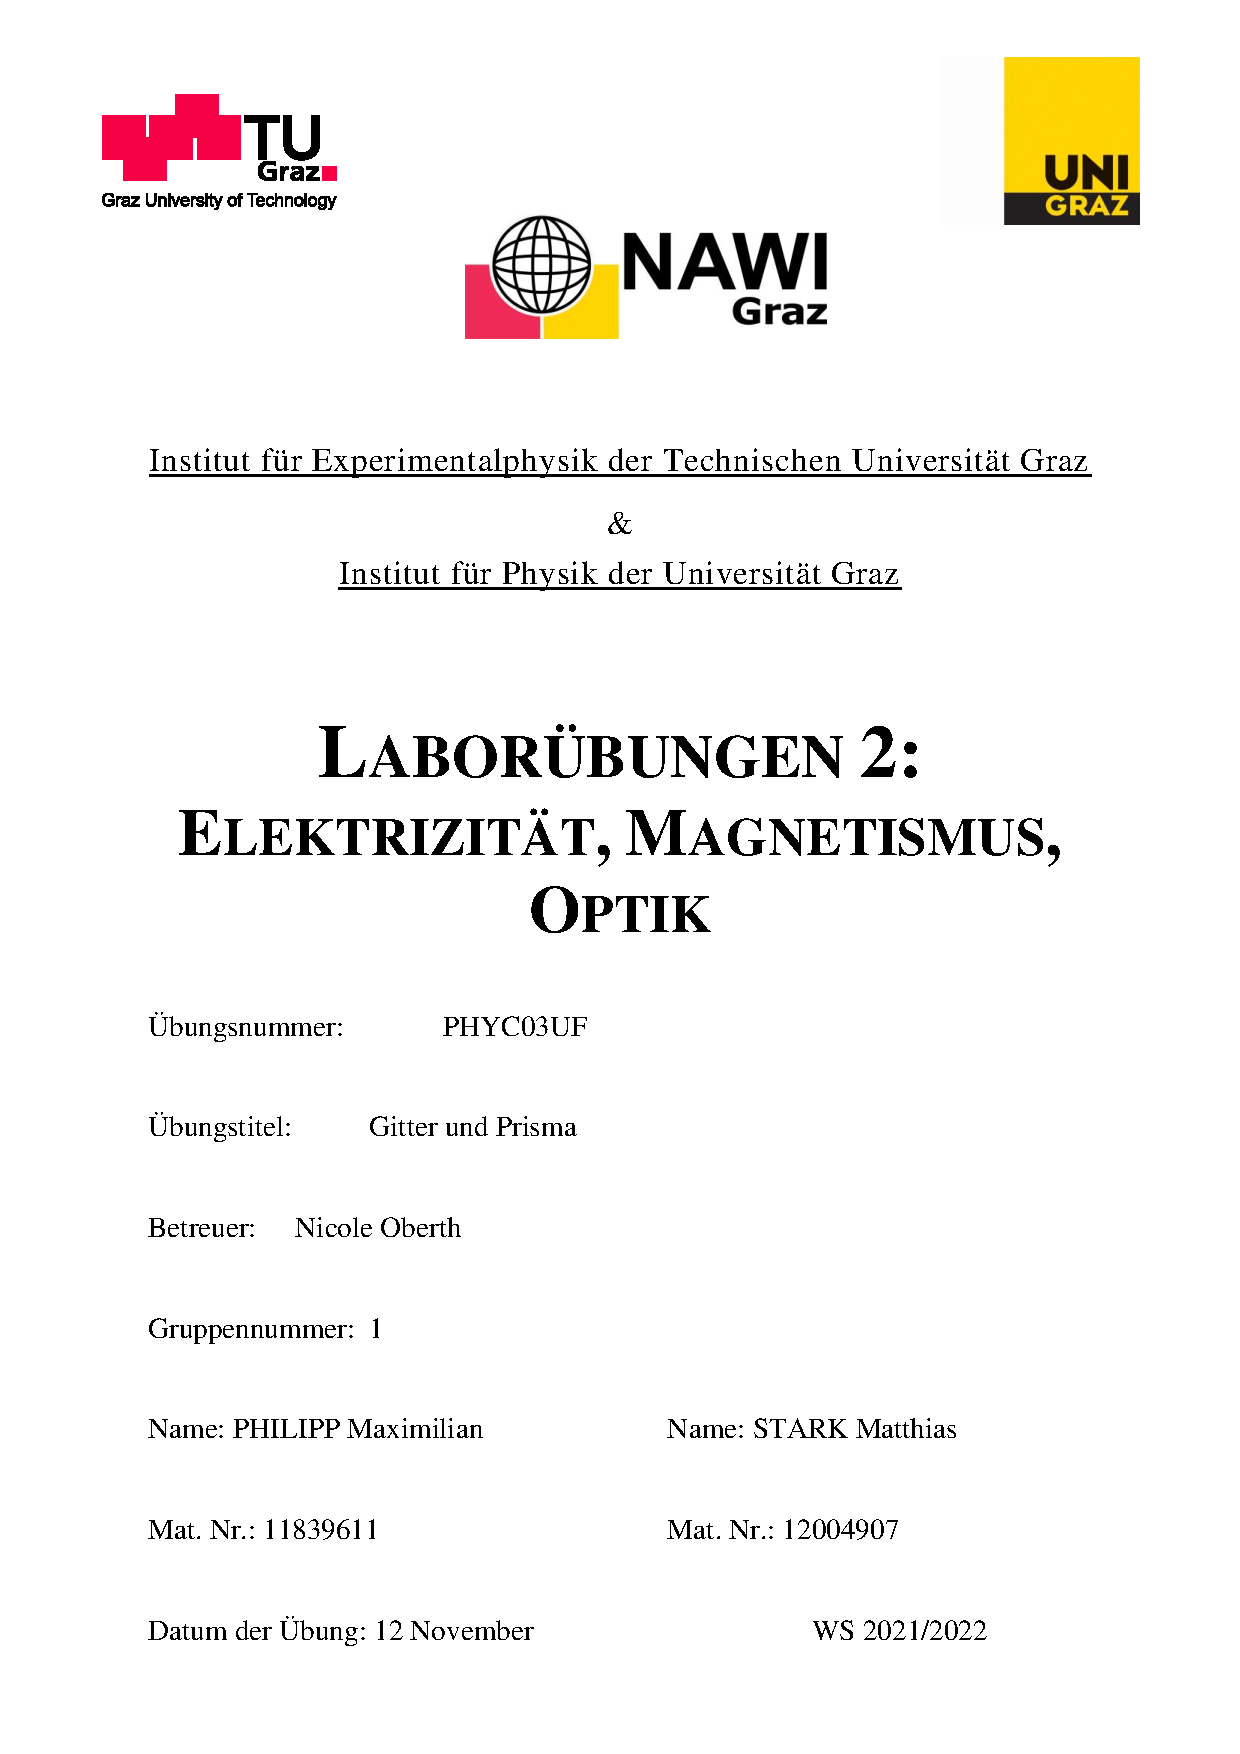
\includepdf{Deckblatt_labor2.pdf}
\tableofcontents
\newpage

\section{Aufgabenstellung\label{Auf0}}

\subsection{Gitter}

\begin{itemize}
	\item Justieren des Spektrometers.

	\item Bestimmung der Gitterkonstante mittels einer Na-Dampflampe.
	      Dabei sind die Wellenlängen der gelben Na-Doppellinien 5889.95 $\mathring{A}$ und 5895.92 $\mathring{A}$.

	\item Bestimmung der Wellenlängen der gut sichtbaren Linien einer Spektrallampe.

	\item Berechnung des Auflösungsvermögens der Messanordnung.

\end{itemize}



\subsection{Prisma}

\begin{itemize}
	\item Justieren des Spektrometers.

	\item Bestimmen Sie den brechenden Winkel des Prismas durch Messung des Reflexionswinkels.
	      Die Messung ist fünfmal zu wiederholen, der Mittelwert für $\gamma$ ist zu berechnen und die
	      Unsicherheit von $\gamma$ mit Hilfe der Messreihe anzugeben.

	\item Bestimmen Sie den Brechungsindex $n(\lambda_0)$ des Prismas für die sichtbaren Linien einer Hg-
	      Dampflampe nach der Methode der minimalen Ablenkung, und zeichnen Sie die Dispersionskurve.
	      Für die kürzeste und längste Wellenlänge ist die Messung 5 mal zu wiederholen.
	      Die relative Unsicherheit der zugehörigen Brechungsindizes ist mittels der Messreihe anzugeben.

	\item Berechnen Sie das Auflösungsvermögen der Messanordnung für eine der beiden gelben
	      Linien mittels der ermittelten Dispersionskurve.

\end{itemize}

\newpage

\section{Grundlagen}

\subsection{Gitter}

\subsubsection{Beugung und Interferenz am Gitter}

Ein ebenes Strichgitter besteht aus lichtdurchlässigen Öffnungen und lichtundurchlässigen Balken,
welche in genau gleichen Abständen abwechselnd aufeinander folgen (\autoref{fig:abb1}).
Praktisch wird ein solches Gitter z.B. durch eine Glasplatte realisiert, in welche mit einem
Diamanten auf einer äußerst präzise arbeitenden Teilungsmaschine genau äquidistante Linien
eingeritzt werden. Ein Gitter ist umso leistungsfähiger, je größer die geteilte Fläche und je kleiner
die regelmäßige Teilung ist. Fällt Licht auf ein solches Gitter, so wird es gebeugt. Von jedem
Punkt einer Öffnung gehen nach dem Huygens’schen Prinzip Kugelwellen aus, die sich je nach
der Richtung und der Wellenlänge durch Interferenz verstärken oder abschwächen. Ein Bündel
parallelen Lichtes falle senkrecht auf das Gitter (\autoref{fig:abb1}). In der Richtung $\varphi$ wird ein Maximum
der Lichtintensität beobachtet, wenn der Gangunterschied $\Delta$ zwischen zwei von benachbarten
Gitteröffnungen ausgehenden Elementarwellen gerade ein ganzes Vielfaches der Wellenlänge $\lambda$
ist.

\begin{minipage}{\textwidth}
	\begin{minipage}[t]{0.5\textwidth}
		\centering
		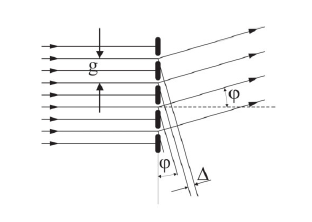
\includegraphics[width=\textwidth]{abb1}
		\captionbelowof{figure}{Paralleles Licht am Gitter. $\Delta = g sin(\varphi)$.}
		\label{fig:abb1}
	\end{minipage}
	\vspace{2mm}
	\begin{minipage}[t]{0.50\textwidth}
		\centering
		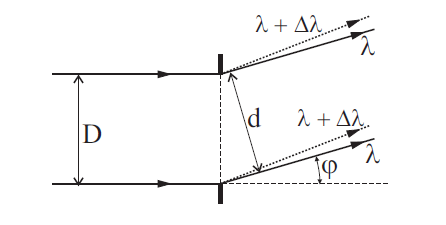
\includegraphics[width=\textwidth]{abb2}
		\captionof{figure}{Zur Benennung der Variablen am Gitter.}
		\label{fig:abb2}
	\end{minipage}
	\vspace{1em}
\end{minipage}

Ist $g$ der Öffnungsabstand, die sogenannte Gitterkonstante, so ist der Gangunterschied:

\begin{equation}
	\Delta = g \textrm{sin}(\varphi)
\end{equation}

Somit lautet die Bedingung für ein Helligkeitsmaximum der Wellenlänge $\lambda$:

\begin{equation}
	z \lambda = g \textrm{sin}(\varphi)
	\label{eq:gitterkonstante}
\end{equation}

$z$ ist eine ganze Zahl, und wird als Ordnungszahl des Beugungsmaximums bezeichnet. Fällt
Licht auf das Gitter, welches sich aus verschiedenen Wellenlängen zusammensetzt, so entsteht
in verschiedenen Richtungen gegen den einfallenden Strahl für jede Wellenlänge ein eigenes
Beugungsmaximum. Eine Folge solcher Maxima, die zu verschiedenen Wellenlängen, d.h. Farben
gehören, bezeichnet man als Spektrum. Den Ordnungszahlen $z = 1, 2, 3, \dots$ entsprechen die
Spektren 1., 2., 3., $\dots$ Ordnung. Sie liegen bei senkrechtem Einfall des Lichtes symmetrisch zur
Einfallsrichtung und entstehen unter umso größerem Winkel $\varphi$, je höher die Ordnungszahl $z$ ist.
Spektren verschiedener Ordnung können sich teilweise überdecken, da nach Gl. (2) zum gleichen
Winkel $\varphi$ Beugungsmaxima verschiedener Ordnung für verschiedene Wellenlängen gehören.

\subsubsection{Dispersion und Auflösungsvermögen des Gitters}

Die Maxima der beiden um $\Delta \lambda$ verschiedenen Wellenlängen $\lambda$ und $\lambda + \Delta \lambda$ werden durch das
Gitter um den Winkel $\Delta \varphi$ getrennt (\autoref{fig:abb2}). Ein Maß für die Auffächerung des Lichtes ist die
Winkeldispersion. Sie ist definiert durch:

\begin{equation}
	\lim_{\Delta \lambda \to 0}  \frac{\Delta \varphi}{\Delta \lambda}= \frac{d \varphi}{d \lambda}
\end{equation}

Für das Gitter erhält man

\begin{equation}
	\frac{d \varphi}{d \lambda} = \frac{z}{g \, \textrm{cos}(\varphi)}
\end{equation}

indem man Gl. (2) nach $\varphi$ differenziert, und den Kehrwert bildet. Eine
ebenfalls wichtige Eigenschaft optischer Geräte ist ihr Auflösungsvermögen.
Dieses gibt für dispergierende Systeme – hier ist es das Gitter – an, welche
Wellenzüge mit der Wellenlänge $\lambda$ und $\lambda + \Delta \lambda$ gerade
noch aufgelöst, d.h. getrennt wahrgenommen werden können. Das
Auflösungsvermögen ist umso größer, je kleiner das beobachtbare $\Delta
	\lambda$ ist, und ist definiert durch $\lambda / \Delta \lambda$. Die Grenze
des optischen Auflösungsvermögens wird beim Gitter nicht nur durch die
Dispersion sondern auch entscheidend durch die Begrenzung des durch das Gitter
hindurchtretenden Strahlenbündels beeinflusst. Das Licht wird nämlich an der
Begrenzung des Bündels gebeugt. Es entsteht daher auch ohne Gitter, allein
durch die begrenzte Breite D des zur Verfügung stehenden Lichtbündels
(\autoref{fig:abb2}) Beugung und Interferenz, und daher eine Folge von Maxima
und Minima. Die stärkste Begrenzung ist nach \autoref{fig:abb2} durch die
Breite $d$ gegeben.

\vspace{2mm}

Das erste Minimum findet man unter dem Winkel $\alpha$, wobei gilt:

\begin{equation}
	\lambda = d \, \sin{ (\alpha)}
\end{equation}

denn die Teilstrahlenbündel 1–6, 2–7, 3–8
usw. (\autoref{fig:abb3}) heben sich gegenseitig auf,
wenn ihr Gangunterschied $(d/2) sin (\alpha)$ gleich
$\lambda/2$ ist.

\begin{figure}[H]
	\begin{center}
		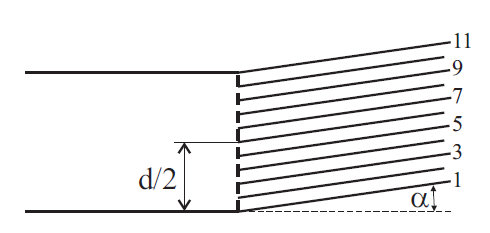
\includegraphics[width=0.5\textwidth]{abb3}
	\end{center}
	\caption{Aufspaltung am Gitter}
	\label{fig:abb3}
\end{figure}

Es ist nicht möglich, das Parallelstrahlenbündel eines Gegenstandpunktes exakt in einem Bildpunkt
zu vereinigen. Das Bild eines Punktes hat vielmehr eine Intensitätsverteilung wie sie
\autoref{fig:abb4} zeigt.
Bei großer Bündelbreite $d$ ist nach Gl. (5) der Abstand des ersten Minimums vom Hauptmaximum
klein, sodass für viele Zwecke die Abbildung punktförmig angesehen werden kann. Wegen
der Kleinheit von $\alpha$ bei großem $d$ kann  $sin (\alpha) \approx \alpha$ gesetzt werden und Gl. (5) durch

\begin{equation}
	\alpha = \frac{\lambda}{d}
\end{equation}

ersetzt werden.

Zwei gegeneinander geneigte Lichtstrahlenbündel werden erfahrungsgemäß dann noch in zwei
getrennt wahrnehmbare Bildpunkte $A$ und $B$ abgebildet, wenn das Hauptmaximum des einen
Punktes mit dem ersten Minimum des zweiten Punktes zusammenfällt. Die Helligkeitskurve $S$
(\autoref{fig:abb5}) als Summe der beiden Intensitätskurven von Punkt $A$ und $B$ zeigt nämlich eine noch
erkennbare Abschwächung in der Mitte. Die Strahlenbündel $A$ und $B$ in \autoref{fig:abb2} können daher
dann noch getrennt beobachtet werden, wenn

\begin{equation}
	\Delta \varphi \geq \alpha
\end{equation}

\begin{minipage}{\textwidth}
	\begin{minipage}[t]{0.33\textwidth}
		\centering
		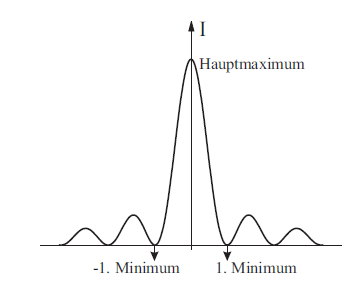
\includegraphics[width=\textwidth]{abb4}
		\captionbelowof{figure}{Intensitätsverlauf eines Lichtbündels am Gitter.}
		\label{fig:abb4}
	\end{minipage}
	\vspace{2mm}
	\begin{minipage}[t]{0.66\textwidth}
		\centering
		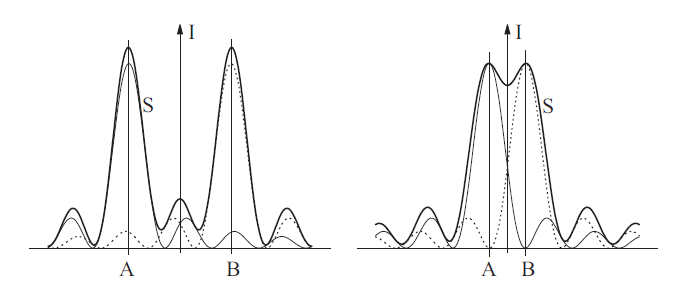
\includegraphics[width=\textwidth]{abb5}
		\captionof{figure}{Intensitätsverläufe zweier gegeneinander geneigter
			Lichtbündel am Gitter, eines an der Auflösungsgrenze. Die
			Punkte werden so lange getrennt wahrgenommen, bis das Maximum
			von $A$ am Ort des ersten Minimums von $B$ ist.}
		\label{fig:abb5}
	\end{minipage}
	\vspace{1em}
\end{minipage}

Da $\Delta \varphi$ durch die Winkeldispersion des Gitters festliegt

\begin{equation}
	\Delta \varphi = \frac{d \varphi}{d \lambda} \Delta \lambda
\end{equation}

erhält man mit Gl. (6):

\begin{equation}
	\frac{\lambda}{\Delta \lambda} = d \, \frac{d \varphi}{d \lambda}
\end{equation}

Die Breite d des gebeugten Bündels hängt vom Winkel $\varphi$ ab, unter dem es das Gitter verläßt
(\autoref{fig:abb2}):

\begin{equation}
	d = D \, \textrm{cos}(\varphi)
\end{equation}

Mit Gl. (4) und (10) nimmt Gl. (9) folgende Gestalt an:

\begin{equation}
	\frac{\lambda}{\Delta \lambda} = \frac{z\, D}{g}
	\label{eq:auflvermgitter}
\end{equation}

$D/g$ stellt die Anzahl $N$ aller vom Licht getroffenen Gitterstriche dar. Man erhält schließlich:

\begin{equation}
	\frac{\lambda}{\Delta \lambda} = z\, N
\end{equation}

Die Größe $\lambda / \Delta \lambda$ wird Auflösungsvermögen genannt. Sie nimmt proportional mit der Strichzahl
$N$ des Gitters und der Ordnung des Spektrums zu.


\subsection{Prisma}

\subsubsection{Brechung und Dispersion}

Der Brechungsindex $n$ eines Mediums ist das Verhältnis der Lichtgeschwindigkeit $c$ im Vakuum
zur Lichtgeschwindigkeit $u$ im Medium:

\begin{equation}
	n = \frac{c}{u}
\end{equation}

Der Gang eines monochromatischen (einfarbigen) Lichtstrahles der Frequenz $\nu$ durch verschiedene,
nicht absorbierende, homogene und isotrope optische Medien wird durch ihre Brechungsindizes,
sowie die geometrische Form und die Lage ihrer Begrenzungsflächen eindeutig festgelegt.
An der Grenze zweier Medien mit verschiedenen Brechungsindizes $n_1$ und $n_2$ tritt stets Reflexion
und Brechung auf (\autoref{fig:abb_1}). Während der reflektierte Strahl $R$ mit dem Lot $L$ stets denselben
Winkel $\alpha$ bildet wie der einfallende Strahl $E$, lässt sich der Winkel $\beta$ zwischen gebrochenem
Strahl $G$ und Lot nach dem Brechungsgesetz von Snellius berechnen.

\begin{equation}
	n_1 \,\textrm{sin}(\alpha) = n_2 \,\textrm{sin}(\beta)
\end{equation}

\begin{minipage}{\textwidth}
	\begin{minipage}[t]{0.5\textwidth}
		\centering
		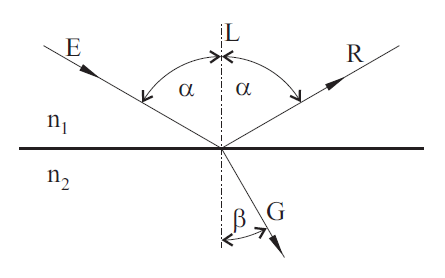
\includegraphics[width=\textwidth]{abb_1}
		\captionbelowof{figure}{Reflexion und Brechung an einer Grenzfläche.}
		\label{fig:abb_1}
	\end{minipage}
	\vspace{2mm}
	\begin{minipage}[t]{0.50\textwidth}
		\centering
		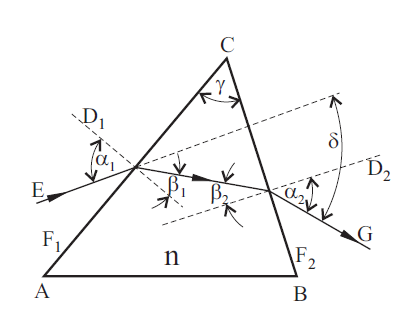
\includegraphics[width=\textwidth]{abb_2}
		\captionof{figure}{Strahlengang im Prisma.}
		\label{fig:abb_2}
	\end{minipage}
	\vspace{1em}
\end{minipage}

Der Berechnungsindex von Vakuum wird willkürlich durch $n_0 = 1$ definiert. Daher tritt der
Lichtstrahl aus dem Vakuum in das zweite Medium so ein, dass

\begin{equation}
	n = \frac{\textrm{sin}(\alpha)}{\textrm{sin}(\beta)}
\end{equation}

gilt.

Diese Form gilt in guter Näherung auch für den Übergang des Lichtes aus einem gasförmigen
Medium in ein flüssiges oder festes, da der Brechungsindex von Gasen nur sehr wenig von 1
verschieden ist. Die Abhängigkeit $n = n(\lambda)$ des Brechungsindex von der Wellenlänge in Luft
(unter Normalbedingungen) bezeichnet man als Dispersionsrelation. Infolge der Dispersion der
Brechungsindizes hängt der Brechungswinkel $\beta$ nicht nur vom Einfallswinkel, sondern auch von
der Wellenlänge des Lichtes ab. Mehrfarbiges Licht wird daher bei der Brechung stets in seine
Bestandteile aufgespalten, d.h. spektral zerlegt.

Als Dispersion $D$ bezeichnet man den Ausdruck

\begin{equation}
	D = \frac{dn}{d\lambda}
\end{equation}

also die Steigung der Dispersionskurve. Das Auflösungsvermögen eines Prismas ist durch

\begin{equation}
	\frac{\lambda}{\Delta \lambda} = t\, \frac{dn}{d\lambda}
\end{equation}

gegeben, mit $t$ der Basislänge des wirksamen Strahlenbündels im Prisma.

\subsubsection{Strahlengang im Prisma}

Diese Übung befasst sich mit dem Strahlengang und der Dispersion eines Glasprismas in Luft
(\autoref{fig:abb_2}). Ein monochromatischer Lichtstrahl $E$ fällt unter dem Winkel $\alpha_1$ auf der einen Seite
$F_1$ (brechende Fläche) des Prismas ein, und verlässt das Prisma nach zweimaliger Brechung
unter dem Winkel $\alpha_2$ aus der Fläche $F_2$. Der Lichtstrahl hat dabei eine Richtungsänderung
um den Winkel $\delta$ erfahren. Der Winkel $\gamma$ zwischen $F_1$ und $F_2$ heißt brechender Winkel. Der
Ablenkungswinkel wird durch den brechenden Winkel $\gamma$ und den Einfallswinkel $\alpha_1$ sowie den
Brechungsindex $n$ bestimmt.

\begin{equation}
	\delta = \delta(\gamma, \alpha_1, n)
\end{equation}

Wegen der Dispersion ist er auch noch von der Farbe des Lichts abhängig. Durch Messung von
$\delta, \gamma, \alpha_1$ bei einer gegebenen Wellenlänge $\lambda$ kann daher

\begin{equation}
	n(\lambda) = f(\delta, \gamma, \alpha_1)
\end{equation}

ermittelt werden, wenn die Funktion $f(\delta, \gamma, \alpha_1)$ bekannt ist. Beim Ein- und Austritt des Strahls
gilt das Brechungsgesetz:

\begin{equation}
	\textrm{sin}(\alpha_1)= n \,\textrm{sin}(\beta_1) \qquad , \qquad \textrm{sin}(\alpha_2)= n \,\textrm{sin}(\beta_2)
\end{equation}

Die Winkel $\alpha_1, \alpha_2, \beta_1, \beta_2, \delta, \gamma$ sind außerdem durch rein geometrische Beziehungen miteinander
verknüpft:

\begin{equation}
	\beta_1 + \beta_2 = \gamma
\end{equation}

\begin{equation}
	\alpha_1 + \alpha_2 = \delta + \gamma
\end{equation}

Die Winkel des Dreiecks $D_1 CD_2$ sind $90^\circ - \beta_1, 90^\circ - \beta_2$ und $\gamma$, und, da die Winkelsumme im
Dreieck $180^\circ$ beträgt, folgt aus $90^\circ - \beta_1 + 90^\circ - \beta_2 + \gamma = 180^\circ$ Gl. (21).
Der Ablenkungswinkel beim Eintritt in das Prisma ist durch $\alpha_1 - \beta_1$ gegeben. Beim Austritt
erfolgt eine weitere Ablenkung um $\alpha_2 - \beta_2$. Die gesamte Ablenkung

\begin{equation}
	\delta = \alpha_1 - \beta_1 + \alpha_2 - \beta_2
\end{equation}

liefert unter Berücksichtigung von Gl. (21) die Beziehung Gl. (22). Um Gl. (18) zu finden, müssen
die Gleichungen (20) (21) (22) verwendet werden. Addiert man die Gleichungen (20), so erhält man
durch trigonometrische Umrechnung:

\begin{equation}
	\textrm{sin}(\alpha_1) + \textrm{sin}(\alpha_2) = 2\, \textrm{sin}\left(\frac{\alpha_1 + \alpha_2}{2}\right) \,\textrm{cos}\left(\frac{\alpha_1 - \alpha_2}{2}\right)
\end{equation}

wegen $\textrm{sin}(\alpha_1) = n \,\textrm{sin}(\beta_1)$ und $\textrm{sin}(\alpha_2) = n \,\textrm{sin}(\beta_2)$ ist:

\begin{equation}
	\textrm{sin}(\alpha_1) + \textrm{sin}(\alpha_2) = n\,(\textrm{sin}(\beta_1) + \textrm{sin}(\beta_2)) = n\,2\, \textrm{sin}\left(\frac{\beta_1 + \beta_2}{2}\right) \,\textrm{cos}\left(\frac{\beta_1 - \beta_2}{2}\right)
\end{equation}

Setzt man Gl. (21) und (22) ein, so gilt

\begin{equation}
	\textrm{sin}\left(\frac{\delta + \gamma}{2}\right) \textrm{cos}\left(\frac{\alpha_1 + \alpha_2}{2}\right) = n\, \textrm{sin}\left(\frac{\gamma}{2}\right) \,\textrm{cos}\left(\frac{\beta_1 - \beta_2}{2}\right)
\end{equation}

oder

\begin{equation}
	\textrm{sin}\left(\frac{\delta + \gamma}{2}\right) = n\, \textrm{sin}\left(\frac{\gamma}{2}\right) \,\frac{\textrm{cos}(\frac{\beta_1 - \beta_2}{2})}{\textrm{cos}(\frac{\alpha_1 + \alpha_2}{2})}
\end{equation}

Um diese Gleichungen auf die Form nach Gl. (18) zu bringen, müsste $\beta_1$, $\beta_2$ und $\alpha_2$ durch $\gamma$, $\delta$,
$\alpha_1$ und $n$ ausgedrückt werden. Dies würde auf eine komplizierte Formel führen. Im Sonderfall
des symmetrischen Strahlenganges

\begin{equation}
	\alpha_1 = \alpha_2 \qquad , \qquad \beta_1 = \beta_2
\end{equation}

erhält man jedoch die einfache Gleichung

\begin{equation}
	n = \frac{\textrm{sin}(\frac{\gamma + \delta}{2})}{\textrm{sin}(\frac{\gamma}{2})}
	\label{eq:brechzahl}
\end{equation}

Der symmetrische Strahlengang ist durch einen minimalen Ablenkungswinkel gekennzeichnet. Es
sei $\alpha_1 > \alpha_2$, dann ist wegen Gl. (21) auch $\beta_1 > \beta_2$. Somit gilt die Ungleichung $\alpha_1 +\beta_1 > \alpha_2 + \beta_2$.
Da eine Ungleichung nach Äquivalenzumformungen erhalten bleibt, gilt auch $\alpha_1 -\alpha_2 > \beta_2 - \beta_1$
und $\textrm{cos}(\alpha_1 -\alpha_2) < \textrm{cos}(\beta_2 - \beta_1)$. Da die Kosinusfunktion symmetrisch ist, gilt:

\begin{equation}
	\textrm{cos}(\alpha_1 -\alpha_2) < \textrm{cos}(\beta_1 - \beta_2)
\end{equation}

Diese Ungleichung gilt auch für $\alpha_1 < \alpha_2$. Der Bruch auf der rechten Seite von Gl. (27) ist daher
im allgemeinen größer als 1. Sein minimaler Wert ist eins bei symmetrischem Strahlendurchgang.
Es hat dann auch die linke Seite von Gl. (27) ein Minimum:

\begin{equation}
	\textrm{sin}\left(\frac{\gamma + \delta}{2}\right) = \textrm{min}
\end{equation}

Da die Sinusfunktion zwischen 0° und 90° monoton steigend ist, kann in diesem Bereich ein
Minimum nur auftreten, wenn das Argument ein Minimum hat: $(\gamma + \delta)/2 = $ min. Der brechende
Winkel liegt fest, somit kann nur der Ablenkungswinkel den minimalen Argumentwert bewirken.

\begin{equation}
	\delta = \textrm{min}
\end{equation}

Für den Bereich 90° bis 270° ist die Sinusfunktion monoton fallend. Ihr Minimum müsste daher
durch ein Maximum des Arguments hervorgerufen werden. Da aber $\gamma + \delta \leq \  180$° $(\alpha_1 \leq \ 90$°), ist
dieser Fall physikalisch nicht realisierbar.

Aufgrund von Gl. (29) lässt sich der Brechungsindex $n$ eines Prismas als Funktion der Wellenlänge
$\lambda$, d.h. der Farbe des Lichts einfach messen, indem man den brechenden Winkel $\gamma$, und für
verschiedene Farben den minimalen Ablenkungswinkel ermittelt:

\begin{equation}
	n (\lambda) = f(\delta,\gamma) \qquad, \qquad \delta = \textrm{min}
\end{equation}

Ein Vergleich mit Gl. (13) zeigt, dass das Aufsuchen der minimalen Ablenkung die Messung des
Einfallswinkel $\alpha_1$ ersetzt.





\newpage

\section{Versuchsanordnung}\label{sec:Versuchsanordnung}

\subsection{Gitter}

Vor den Spalt $SP$ des Kollimatorrohres $K$ eines Spektrometers (\autoref{fig:abb6}) wird eine Lichtquelle $L$
gebracht. Das vom Kollimator kommende Parallelstrahlenbündel wird am Gitter $G$ gebeugt, und
die Interferenzbilder im Fernrohr $F$ beobachtet. Der Spektrometertisch $T$ besitzt eine Gradeinteilung
W, sodass die Stellung des Fernrohres mit Hilfe eines Nonius $N$ abgelesen werden kann.
Der Nonius ist mit dem Fernrohr verbunden. Er enthält 10 Teilstriche auf einer Teilungslänge
von 9 Skalenteilen. Dadurch unterscheiden sich die beiden Skalen $W$ und $N$ um 0.1 Teilstrich
pro Skalenteil. Deckt sich der i-te Teilstrich des Nonius mit einem Skalenstrich der Teilung W,
so bedeutet dies, dass $0.1i$ Skalenteile zum Skalenwert $c$ hinzuzuzählen sind.

Zur Bestimmung der Gitterkonstanten bringt man eine Lichtquelle bekannter Wellenlänge vor
den Spalt des Kollimators, und misst den Ablenkungswinkel $\varphi$. Die Messung wird mit zunehmender
Ordnung $z$ genauer, denn die relative Unsicherheit von $\varphi$ verkleinert sich mit zunehmendem
Winkel, da man in jeder Stellung mit einer gleichbleibenden Ableseunsicherheit $\Delta \varphi$
rechnen kann. Durch Wahl von $z$ und Messung des Winkels $\varphi$ kann nach Gl. (1) bei bekannter
Wellenlänge die Gitterkonstante berechnet werden. Bei bekannter Gitterkonstante $g$ kann nun
Gl. (1) zur Wellenlängenmessung benützt werden.

\begin{figure}[H]
	\begin{center}
		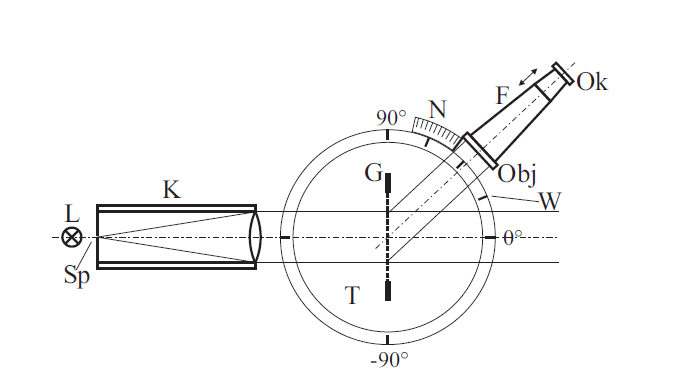
\includegraphics[width=0.8\textwidth]{abb6}
	\end{center}
	\caption{Aufbau zur Messung mit dem Gitter.}
	\label{fig:abb6}
\end{figure}

\newpage

\subsection{Prisma}

\subsubsection{Messung des brechenden Winkels}

Das Prisma wird so auf den fixierten Spektrometertisch $T$ gestellt, dass der zu messende Winkel
$\gamma$ auf das Spaltrohr $K$ hinweist (\autoref{fig:abb_3}). Dann wird das Fernrohr $F$ abwechselnd nach links
und nach rechts so weit geschwenkt, bis man das Spiegelbild des mit der Lampe $L$ beleuchteten
Spaltes Sp im Fernrohr sieht, und mit dem Fadenkreuz zusammenfällt. Man liest die zugehörigen
Stellungen der reflektierten Spaltbilder $S_1$ und $S_2$ an der Winkelteilung W des Spektrometertisches
mit Hilfe des Nonius N ab. Durch diese beiden Ablesungen ist der Winkel zwischen den
beiden reflektierten Strahlenbündeln bestimmt. Aus der geometrischen Anordnung und dem
Reflexionsgesetz: Einfallswinkel = Reflexionswinkel folgt:

\begin{equation}
	\gamma = \frac{\epsilon}{2}
	\label{eq:gamma}
\end{equation}

\begin{minipage}{\textwidth}
	\begin{minipage}[t]{0.5\textwidth}
		\centering
		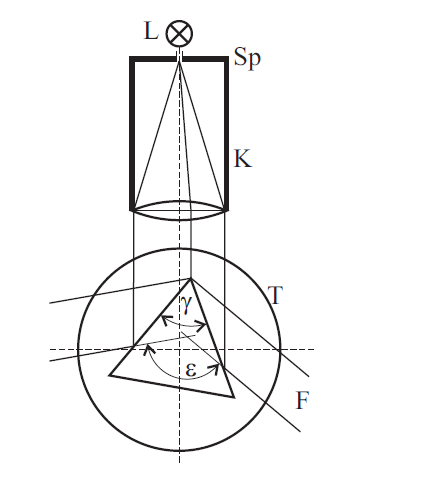
\includegraphics[width=\textwidth]{abb_3}
		\captionbelowof{figure}{Messung des brechenden Winkels.
			L Lampe, Sp Spalt, K Kollimator, T
			Teilkreis, F zum Fernrohr.}
		\label{fig:abb_3}
	\end{minipage}
	\vspace{2mm}
	\begin{minipage}[t]{0.50\textwidth}
		\centering
		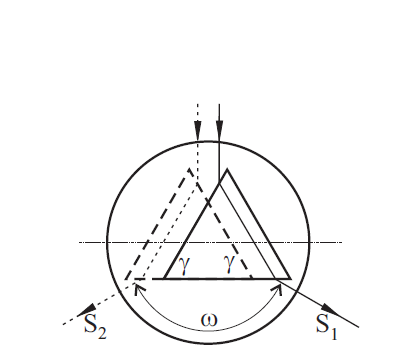
\includegraphics[width=\textwidth]{abb_4}
		\captionof{figure}{Messung des minimalen Ablenkungswinkels.}
		\label{fig:abb_4}
	\end{minipage}
	\vspace{1em}
\end{minipage}


\subsubsection{Messung des minimalen Ablenkungswinkels}

Man stellt das Prisma so auf den Spektrometertisch, dass das vom Spaltrohr kommende Licht auf
eine der brechenden Flächen $F_1$ und $F_2$ einfällt, und sucht den gebrochenen Strahl. Man dreht
nun das Prisma langsam und verfolgt die Bewegung des gebrochenen Strahles mit dem Fernrohr.
Im Moment, in dem die Stellung minimaler Ablenkung durchlaufen wird, kehrt der Drehsinn
des gebrochenen Strahles um. Durch Hin- und Herschwenken des Prismas lässt sich die genaue
Minimumeinstellung sehr leicht feststellen. Diese besondere Lage $S_1$ des gebrochenen Strahles
wird an der Winkelteilung des fixierten Spektrometertisches abgelesen (\autoref{fig:abb_4}). Man könnte
nun das Prisma entfernen, und mit dem Fernrohr den ungebrochenen Strahl $S_0$ aufsuchen. Der
Winkel $\delta$ zwischen diesen Lagen ist der gesuchte Ablenkungswinkel. Man führt die Messung
jedoch besser in zwei zum einfallenden Strahl symmetrischen Lagen des Prismas durch. Man
dreht daher das Prisma bei fixiertem Spektrometertisch, bis das Licht auf die zweite brechende
Fläche fällt, und sucht wieder die Lage minimaler Ablenkung $S_2$. Der Winkel $\omega$ zwischen diesen
beiden Lagen ist aus Symmetriegründen gleich der doppelten minimalen Ablenkung. Es gilt daher:

\begin{equation}
	\delta = \frac{\omega}{2}
\end{equation}

Diese Methode liefert genauere Werte für $\delta$. Die absolute Unsicherheit der Winkelmessung kann
bei beiden Methoden gleich angenommen werden, der relative Unsicherheit der Messung von $\omega$
ist jedoch halb so groß.

\vspace{2mm}

\newpage

Der Tatsächliche Versuchsaufbau ist in folgender Abbildung ersichtlich.

\begin{figure}[H]
	\begin{center}
		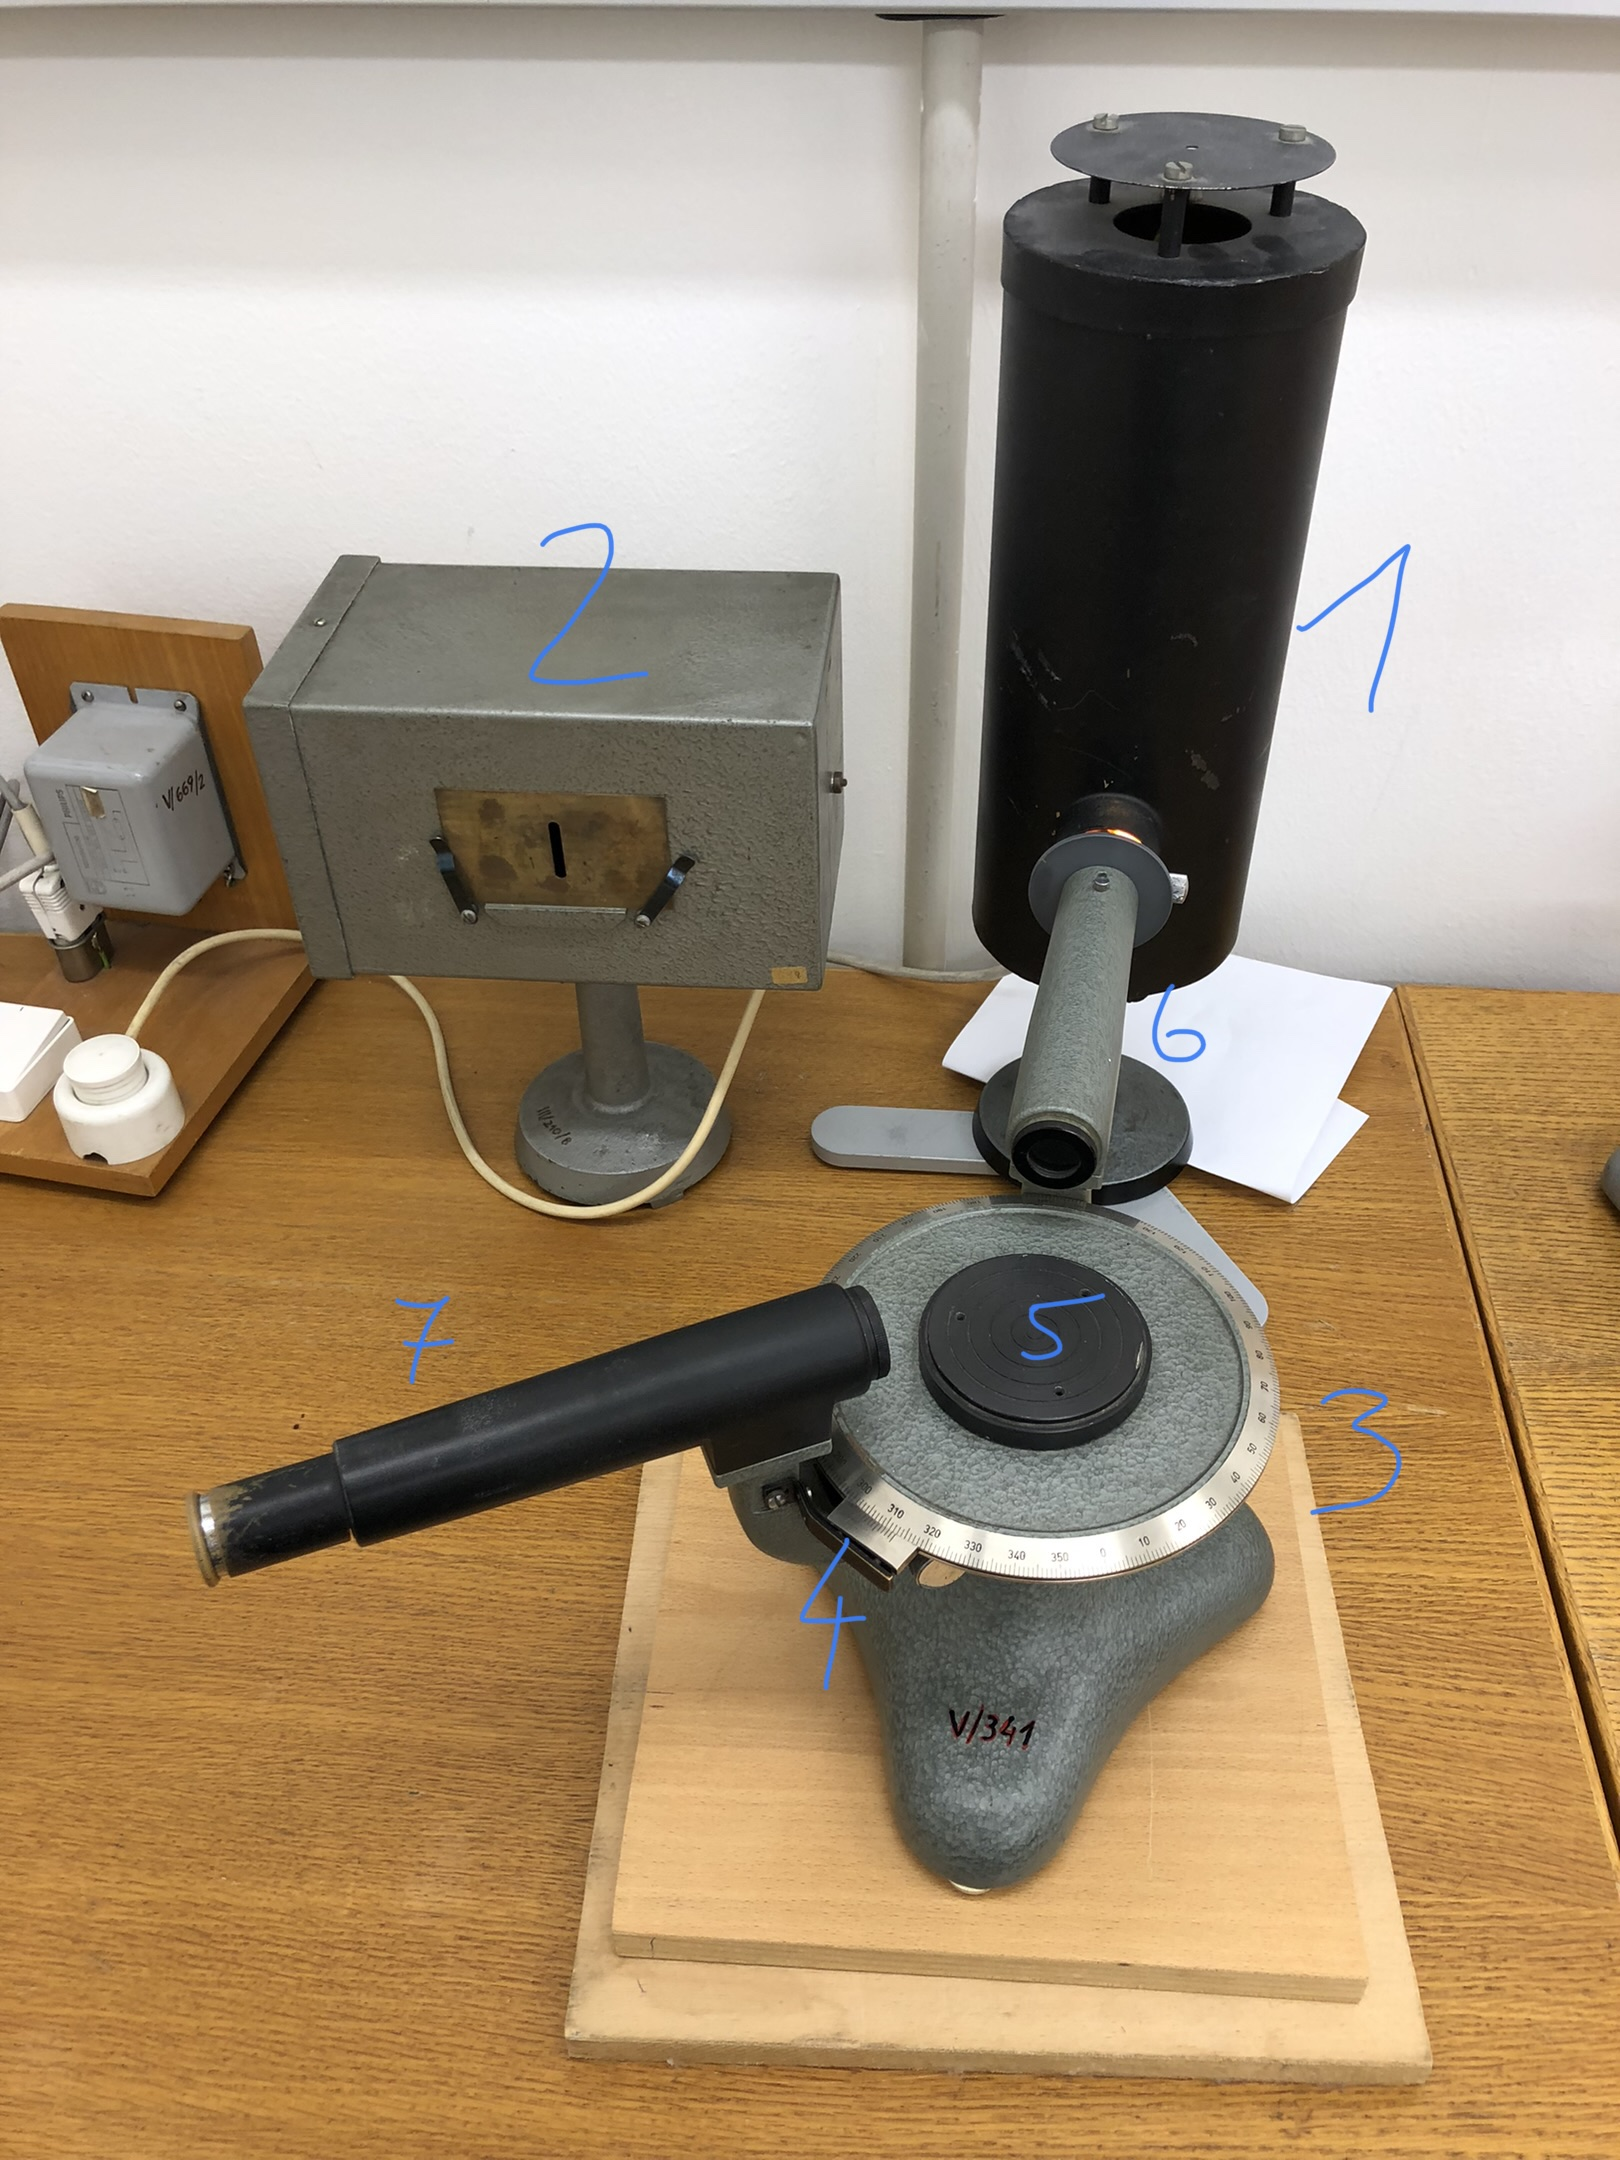
\includegraphics[width=0.6\textwidth]{aufbau_eig}
	\end{center}
	\caption{Versuchsaufbau, 1 beschreibt dabei die Na-Dampflampe, 2 die Spektrallampe, 3 dein Spektrometertisch, auf den sich die Gradeinteilung mit Nonius (4) und das Podest für das Gitter und Prisma (5) befindet, 6 der Kollimator und 7 das Fernrohr.}
	\label{fig:aufbau}
\end{figure}

Das verendete Beugungsgitter und Prisma sind in folgender Abbildung sichtbar.

\begin{figure}[H]
	\begin{center}
		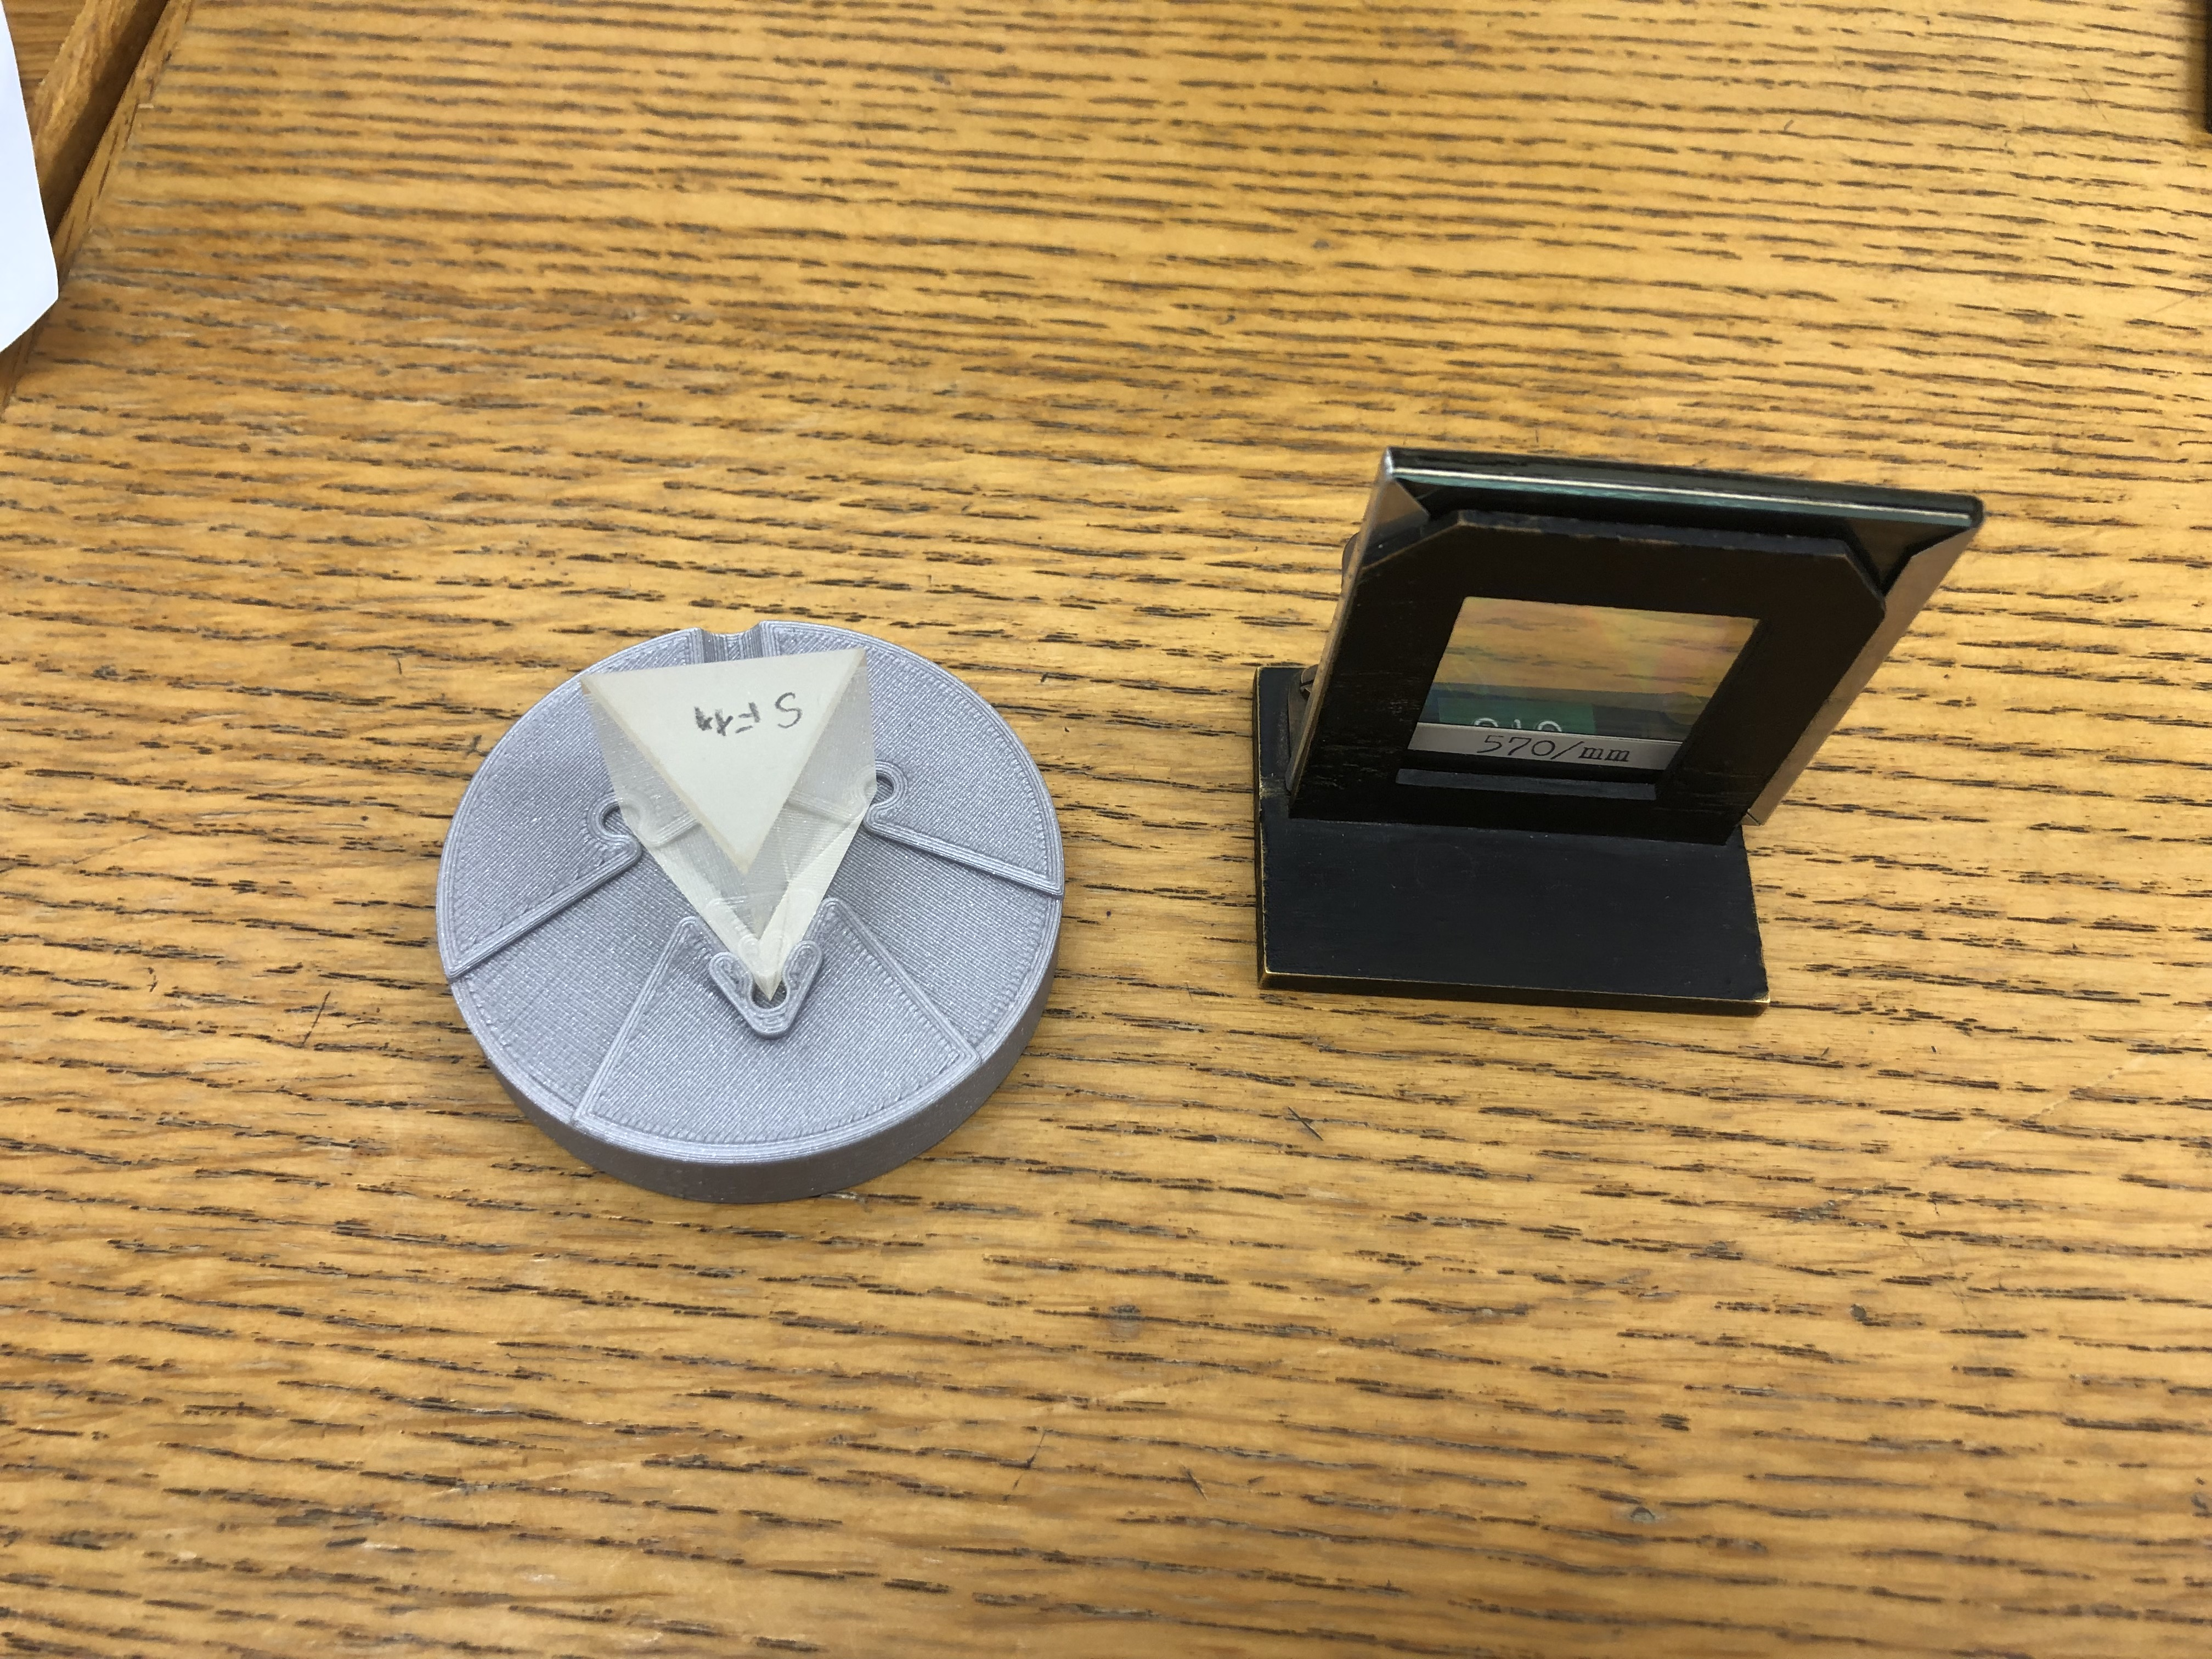
\includegraphics[width=0.4\textwidth]{prisma}
	\end{center}
	\caption{Verwendetes Beugungsgitter und Prisma}
	\label{fig:prisma}
\end{figure}

\section{Geräteliste}

\noindent Für die Messungen wurden folgende Geräte verwendet:

\captionof{table}{Verwendete Geräte }
\begin{center}
	\begin{tabular}{|c|c|c|c|} \hline
		\textbf{Gerät}         & \textbf{Typ}               & \textbf{Hersteller} \\ \hline

		Na-Dampflampe          & SO 40 35 60-35 W (V/615/1) & Philips             \\ \hline
		Spektrallampe          & 58230AH/00                 & Philips             \\ \hline
		Beugungsgitter         & G / 8                      &                     \\ \hline
		Prisma                 & S F 11                     &                     \\ \hline
		Spektrometertisch      & V / 341                    &                     \\ \hline
		Spalt                  &                            &                     \\ \hline
		Fernrohr               &                            &                     \\ \hline
		Gradanzeige mit Nonius &                            &                     \\ \hline
		Kollimator             &                            &                     \\ \hline
		Millimeterpapier       &                            &                     \\ \hline
		Karte                  &                            &                     \\ \hline
	\end{tabular}
\end{center}



\section{Versuchsdurchführung \& Messergebnisse}\label{sec:Versuchsdurchführung}

Sofern es nicht anders angegeben ist, ist bei allen Winkelangaben von einer Unsicherheit von
$\pm$\SI{0.2}{\degree} auszugehen.

\subsection{Gitter}

\subsubsection{Gitterkonstante}

Zunächst wird die Gitterkonstante des verwendeten Beugungsgitters bestimmt. Dazu wird die NA-Dampflampe als Lichtquelle für die Anordnung verwendet, weil diese annähernd monochromatisches Licht einer bekannten Wellenlänge aussendet. Der Mittelwert der Wellenlänge der Kennlinien beträgt laut Angabe \SI{589.2935}{\nm} \cite{gitterprismavorlage}.

\vspace{2mm}

Bei der NA-Dampflampe ist dabei zu beachten, dass diese bereits einige Minuten läuft, um dafür zu sorgen, dass ein konstantes Spektrum ausgestrahlt wird. Nun wird der Kollimator vor die Lichtquelle platziert, wie auch in \autoref{fig:aufbau} sichtbar, und der Spalt so weit geschlossen, dass gerade noch eine scharfe Linie sichtbar wird. Nun wird der Winkel, unter welchem das Licht gebeugt wird, bestimmt. Dazu wird die $\pm$ 2. Ordnung mit dem Fernrohr gesucht und mit den sich darin befindenden Fadenkreuz anvisiert, wie in \autoref{fig:gitter} ersichtlich.

\begin{figure}[H]
	\begin{center}
		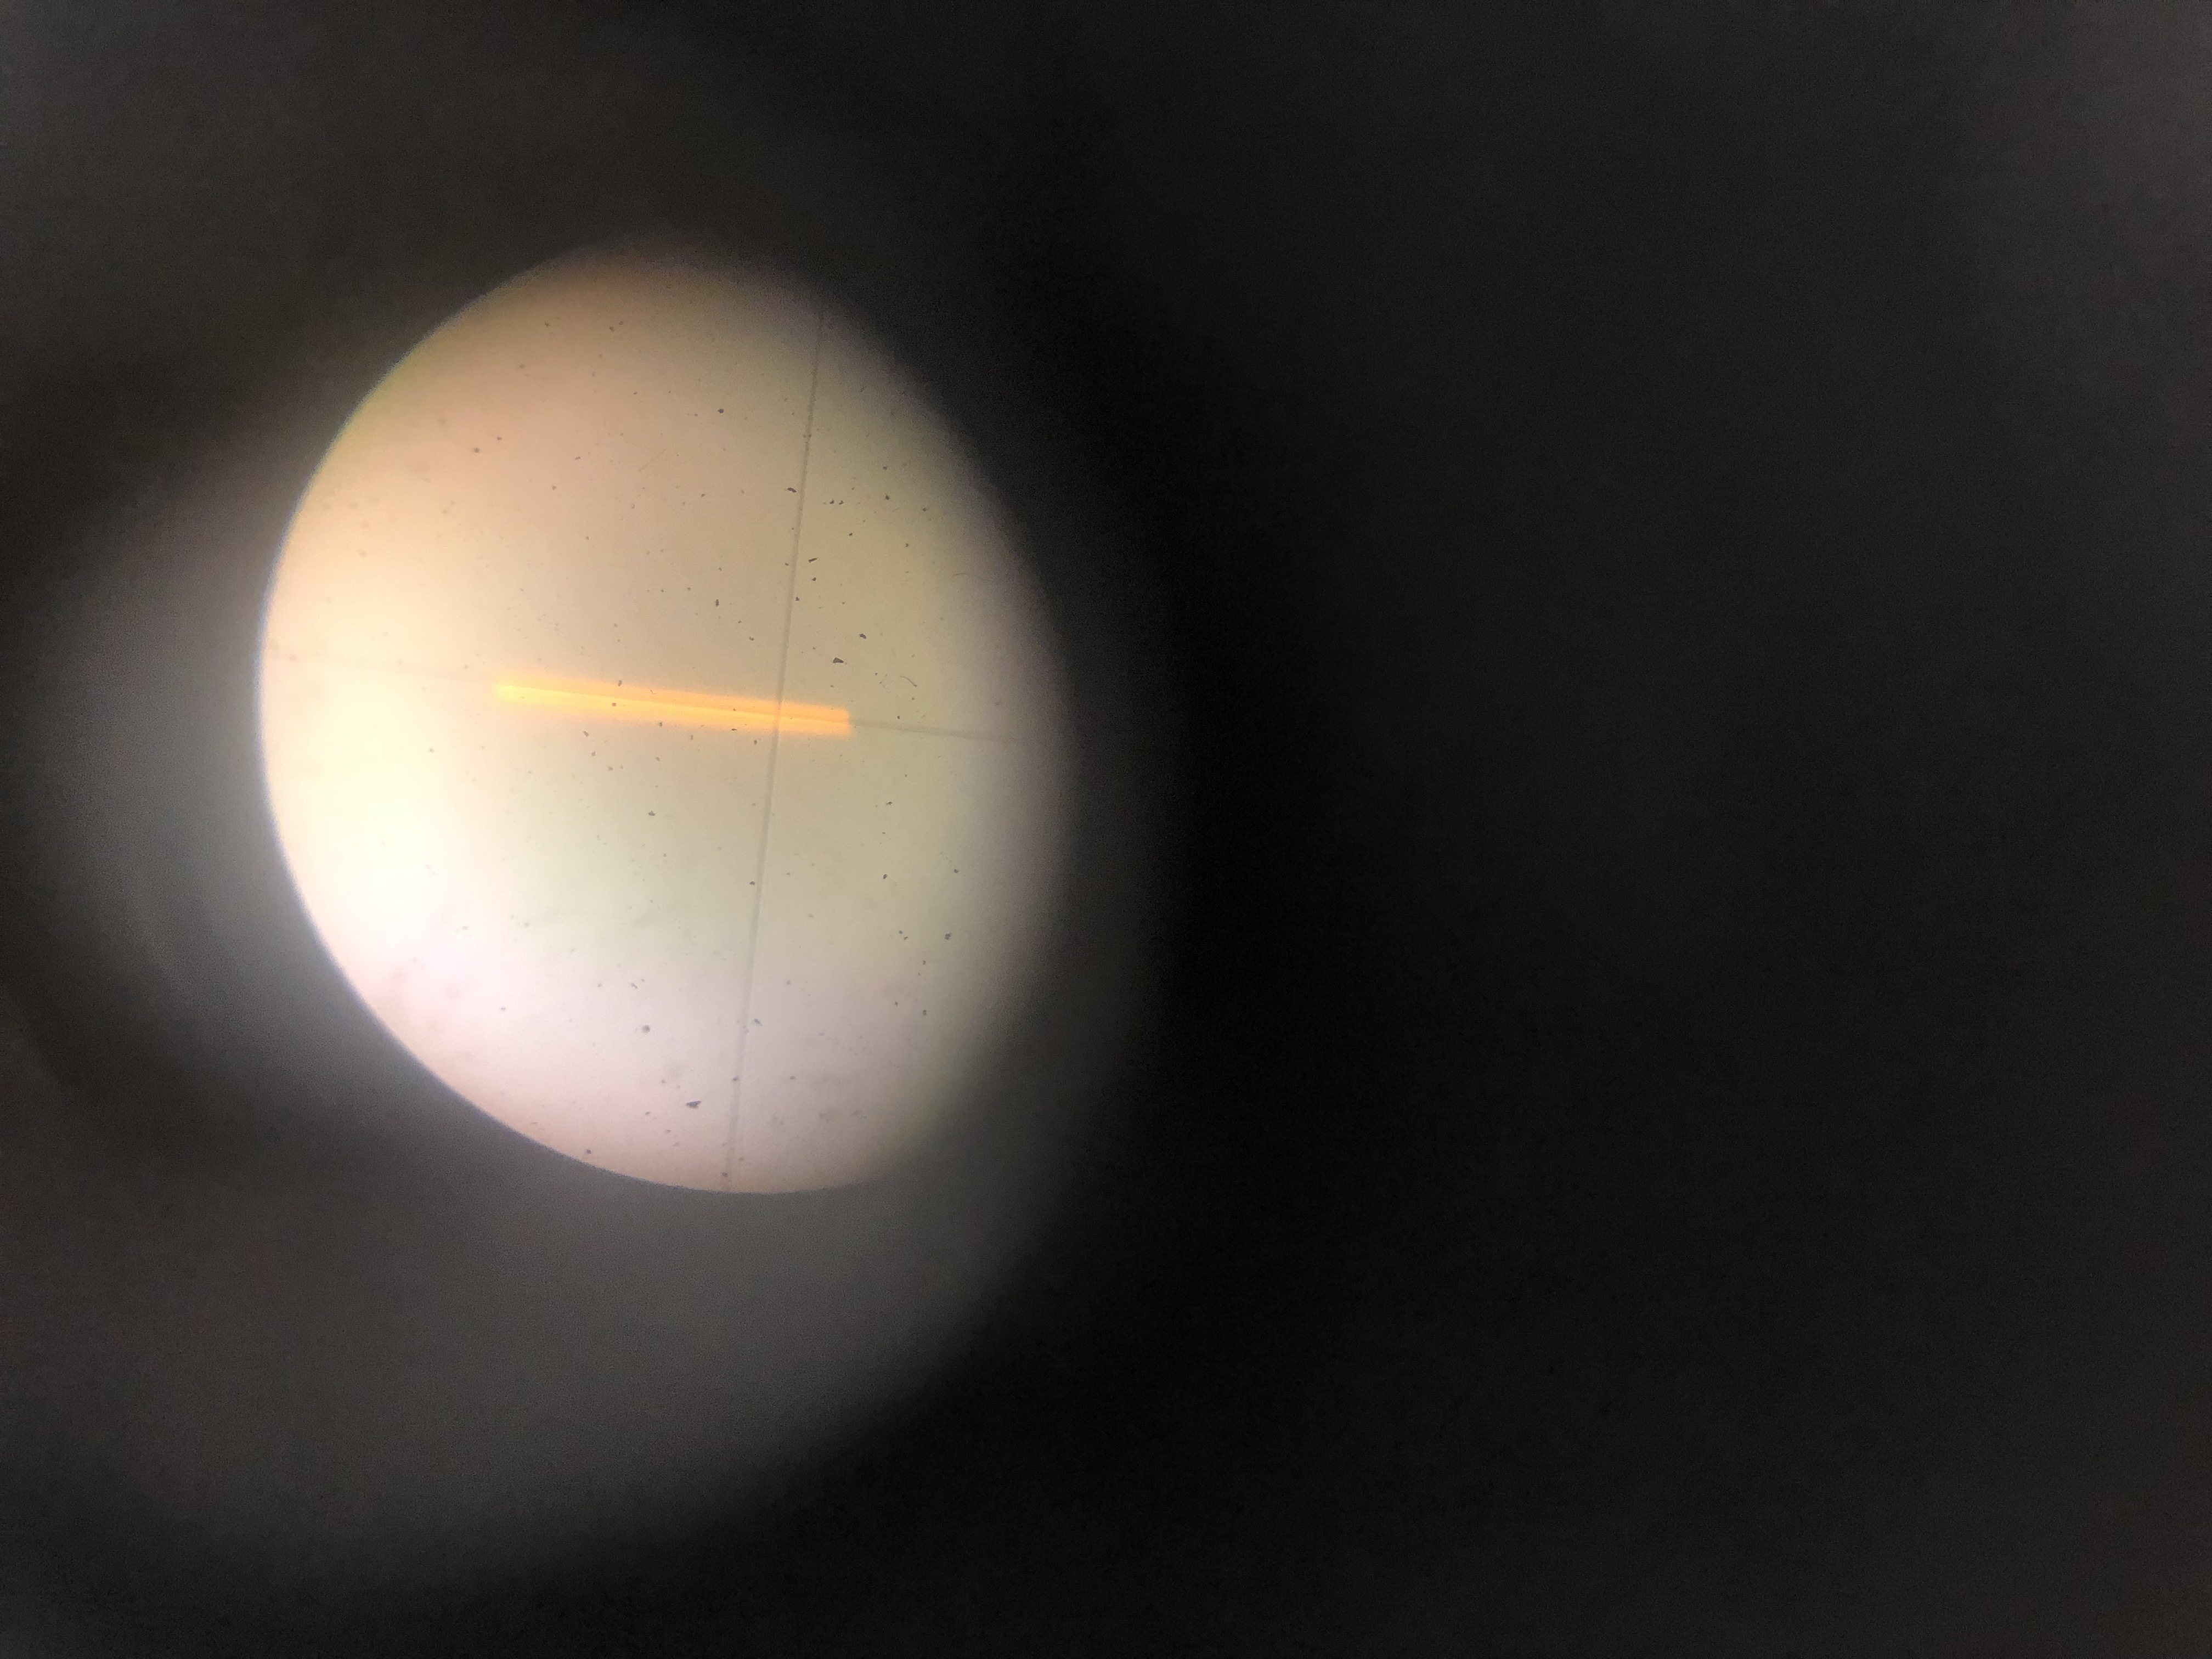
\includegraphics[angle=-90,width=0.4\textwidth]{gitter}
	\end{center}
	\caption{mit Fadenkreuz anvisierte Beugungsordnung}
	\label{fig:gitter}
\end{figure}


Dadurch kann der entsprechende Winkel an der Gradeinteilung des Tisches
abgelesen werden. Um einen Fehler durch eine eventuelle Verschiebung des
Fadenkreuzes auszuschließen wird, wie bereits erwähnt, der Winkel der positiven
und negativen Beugungsordnung notiert und der Mittelwert für die Berechnung
verwendet. Diese Messung wird insgesamt 6 mal wiederholt, was folgende Werte
liefert.

\begin{table}[H]
	\caption{gemessene Werte der Winkel Na-Dampflampe \\ $\varphi_r \dots$ abgelesener Winkel nach rechts \\ $\varphi_l \dots$ abgelesener Winkel nach links}
	\label{tab:messwinkelnadampf}
	\centering
	\begin{tabular}{lrr}
\toprule
{} &  $\varphi_r$ / \si{\degree} &  $\varphi_l$ / \si{\degree} \\
\midrule
0 &                        42.1 &                       317.3 \\
1 &                        42.0 &                       317.4 \\
2 &                        41.9 &                       317.4 \\
3 &                        42.0 &                       317.3 \\
4 &                        42.0 &                       317.3 \\
5 &                        41.9 &                       317.2 \\
\bottomrule
\end{tabular}

\end{table}

\newpage

\subsubsection{Wellenlänge}

Um die Wellenlängen der unterschiedlichen Farben zu bestimmen, wird die Na-Dampflampe durch die Spektrallampe ersetzt und die Apparatur wieder, wie bereits zuvor beschrieben aufgebaut.

Nun wird der Winkel der einzelnen Farben der 2. Beugungsordnung bestimmt, indem wieder das Fadenkreuz des Fernrohrs auf der entsprechenden Linie zentriert wird, wie beispielsweise in \autoref{fig:wellenl_g} sichtbar.

\begin{figure}[H]
	\begin{center}
		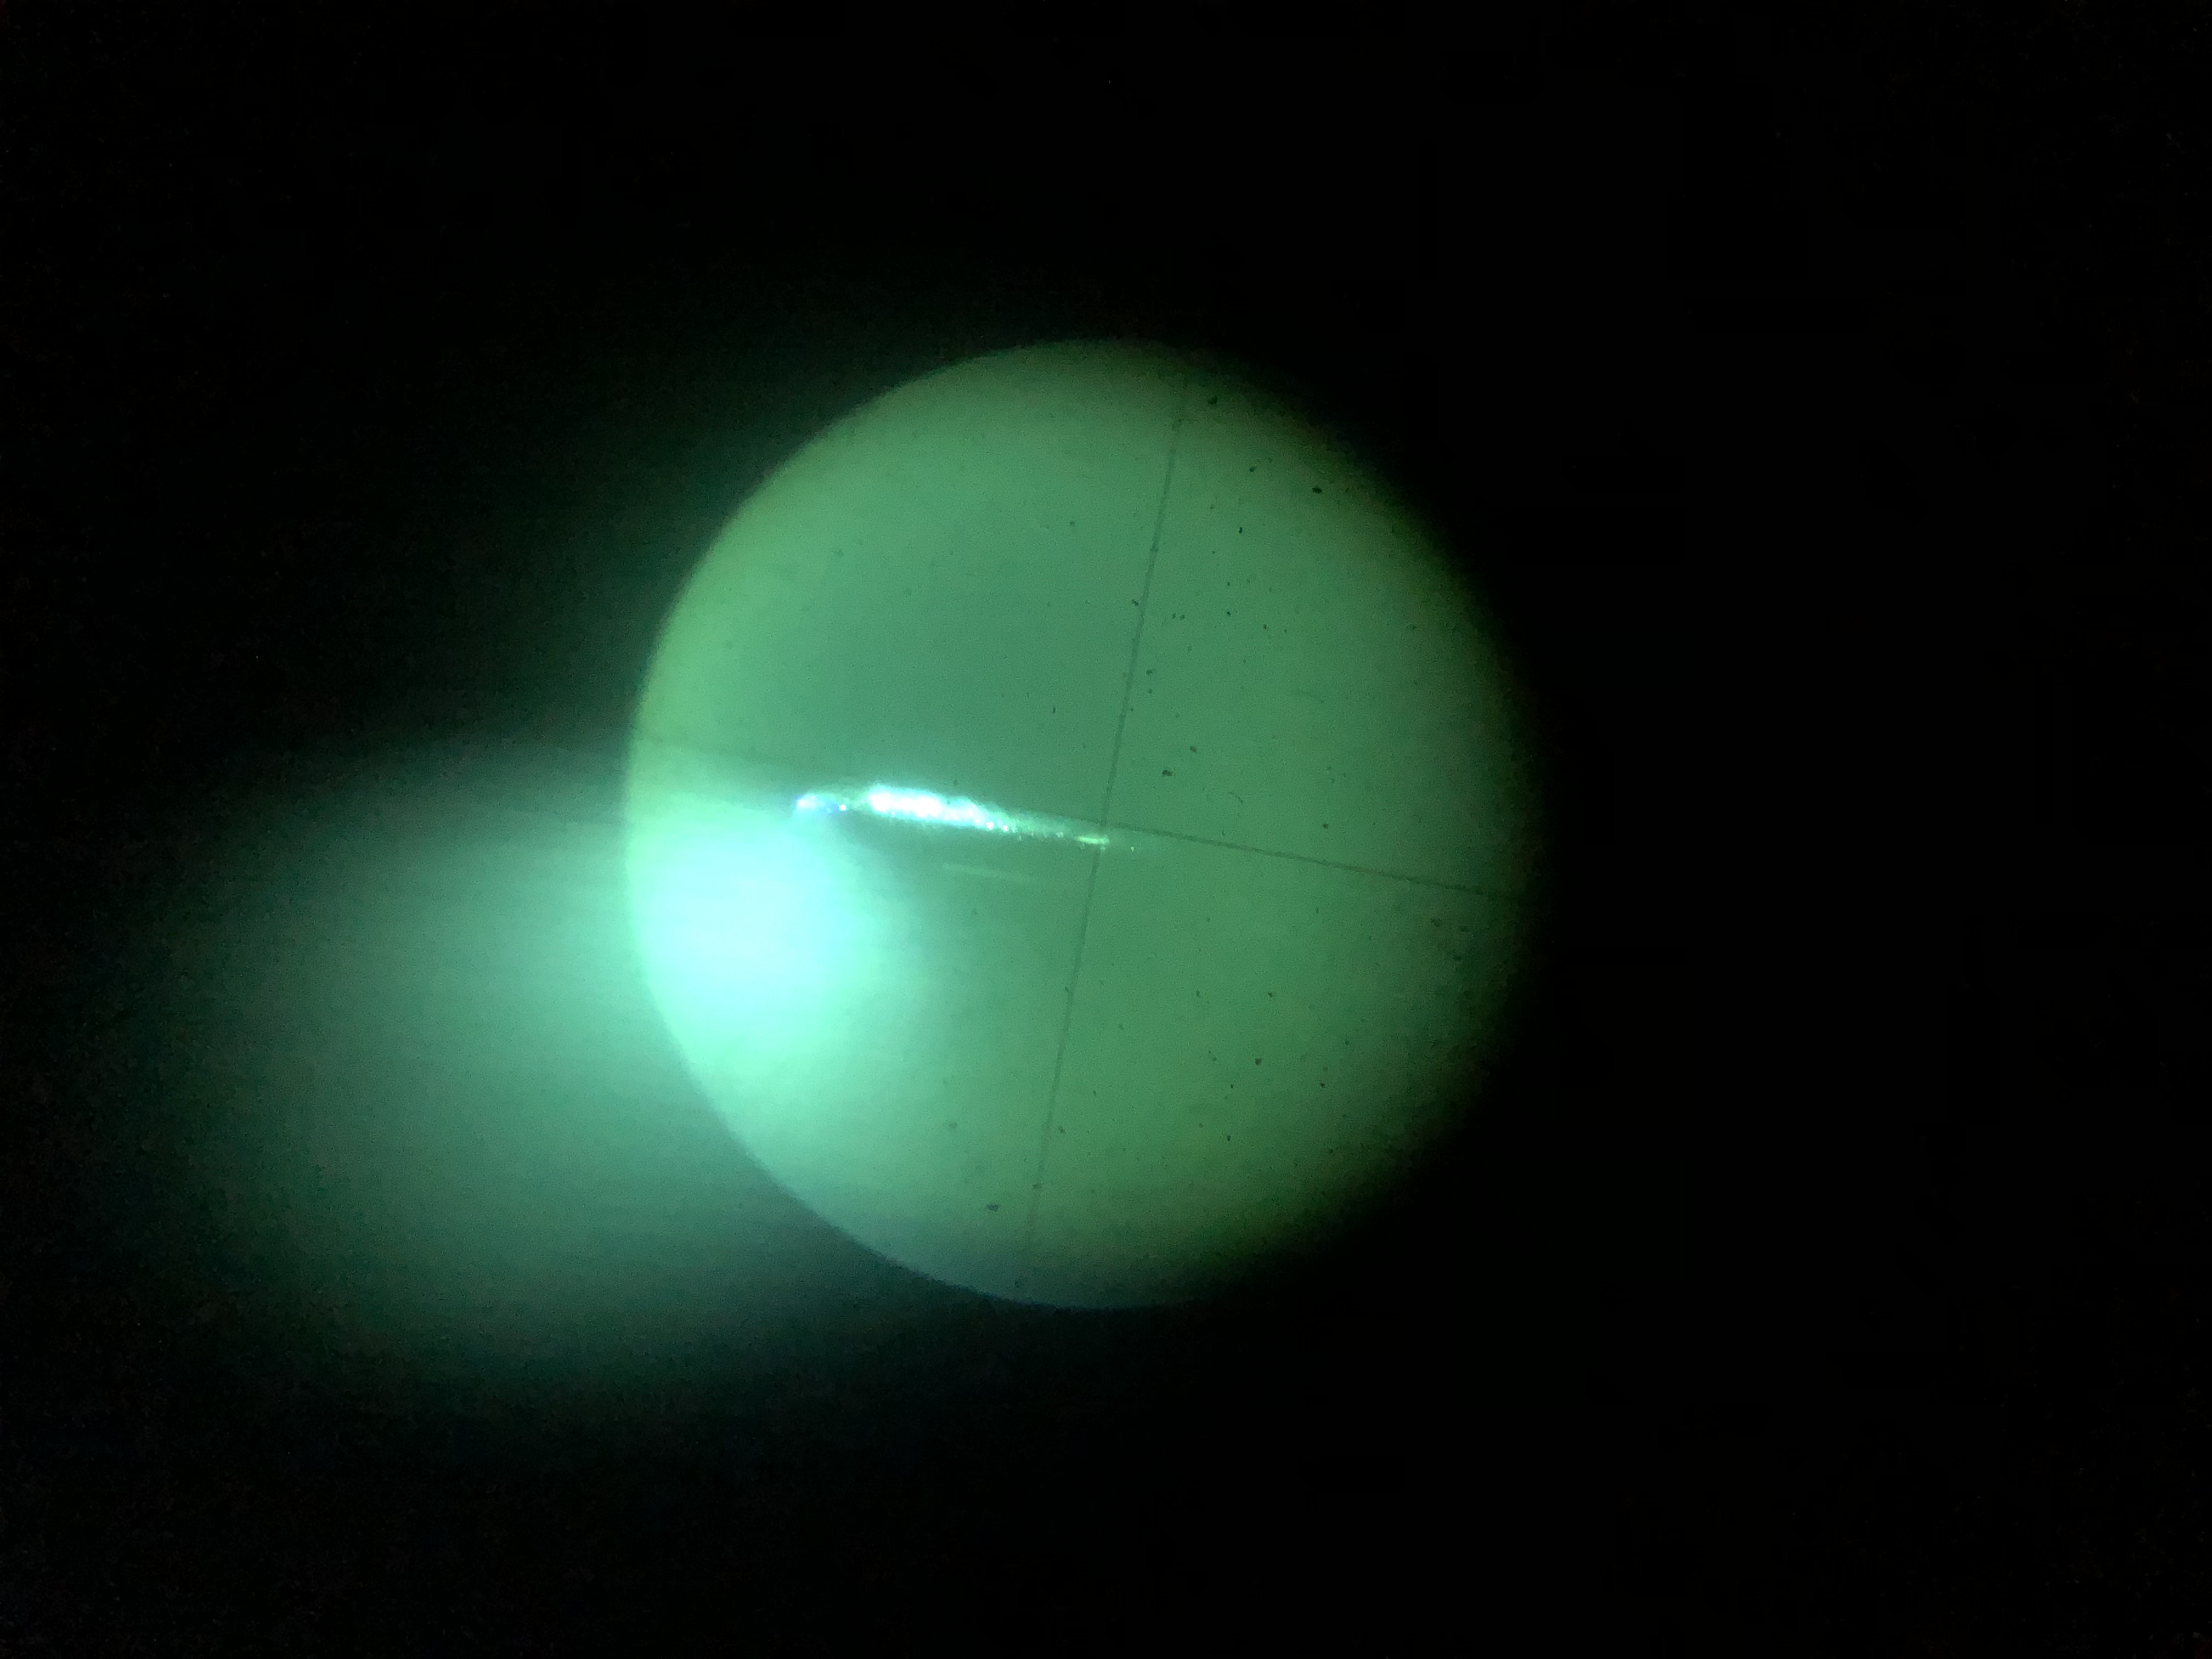
\includegraphics[angle=-90,width=0.4\textwidth]{wellenl_g}
	\end{center}
	\caption{anvisieren der unterschiedlichen Farben mithilfe des Fadenkreuzes}
	\label{fig:wellenl_g}
\end{figure}

Die so erhaltenen Werte für die Winkel sind in folgender Tabelle aufgelistet.

\begin{table}[H]
	\caption{gemessene Winkel der verschiedenen Wellenlängen\\ $\varphi_r \dots$ abgelesener Winkel nach rechts \\ $\varphi_l \dots$ abgelesener Winkel nach links}
	\label{tab:messwinkelwellenlange}
	\centering
	\begin{tabular}{lrr}
	\toprule
	{}      & $\varphi_r$ / \si{\degree} & $\varphi_l$ / \si{\degree} \\
	\midrule
	Violett & 27.5                       & 332.3                      \\
	Blau    & 29.8                       & 330.0                      \\
	Türkis1 & 34.1                       & 325.6                      \\
	Türkis2 & 34.6                       & 325.3                      \\
	Grün    & 38.5                       & 321.2                      \\
	Orange1 & 41.1                       & 318.5                      \\
	Orange2 & 41.4                       & 318.3                      \\
	Rot1    & 43.9                       & 315.8                      \\
	Rot2    & 45.3                       & 314.2                      \\
	\bottomrule
\end{tabular}

\end{table}


\subsubsection{Auflösungsvermögen}

Um das Auflösungsvermögen der Anordnung bestimmen zu können muss der Durchmesser des Kollimators bestimmt werden. Dazu wird Millimeterpapier vor den Kollimator gehalten, wodurch so durch abzählen der Kästchen der Durchmesser des Lichtkreises bestimmt werden kann. Die entsprechende Vorgehensweise ist in folgender \autoref{fig:mmp} sichtbar.

\begin{figure}[H]
	\begin{center}
		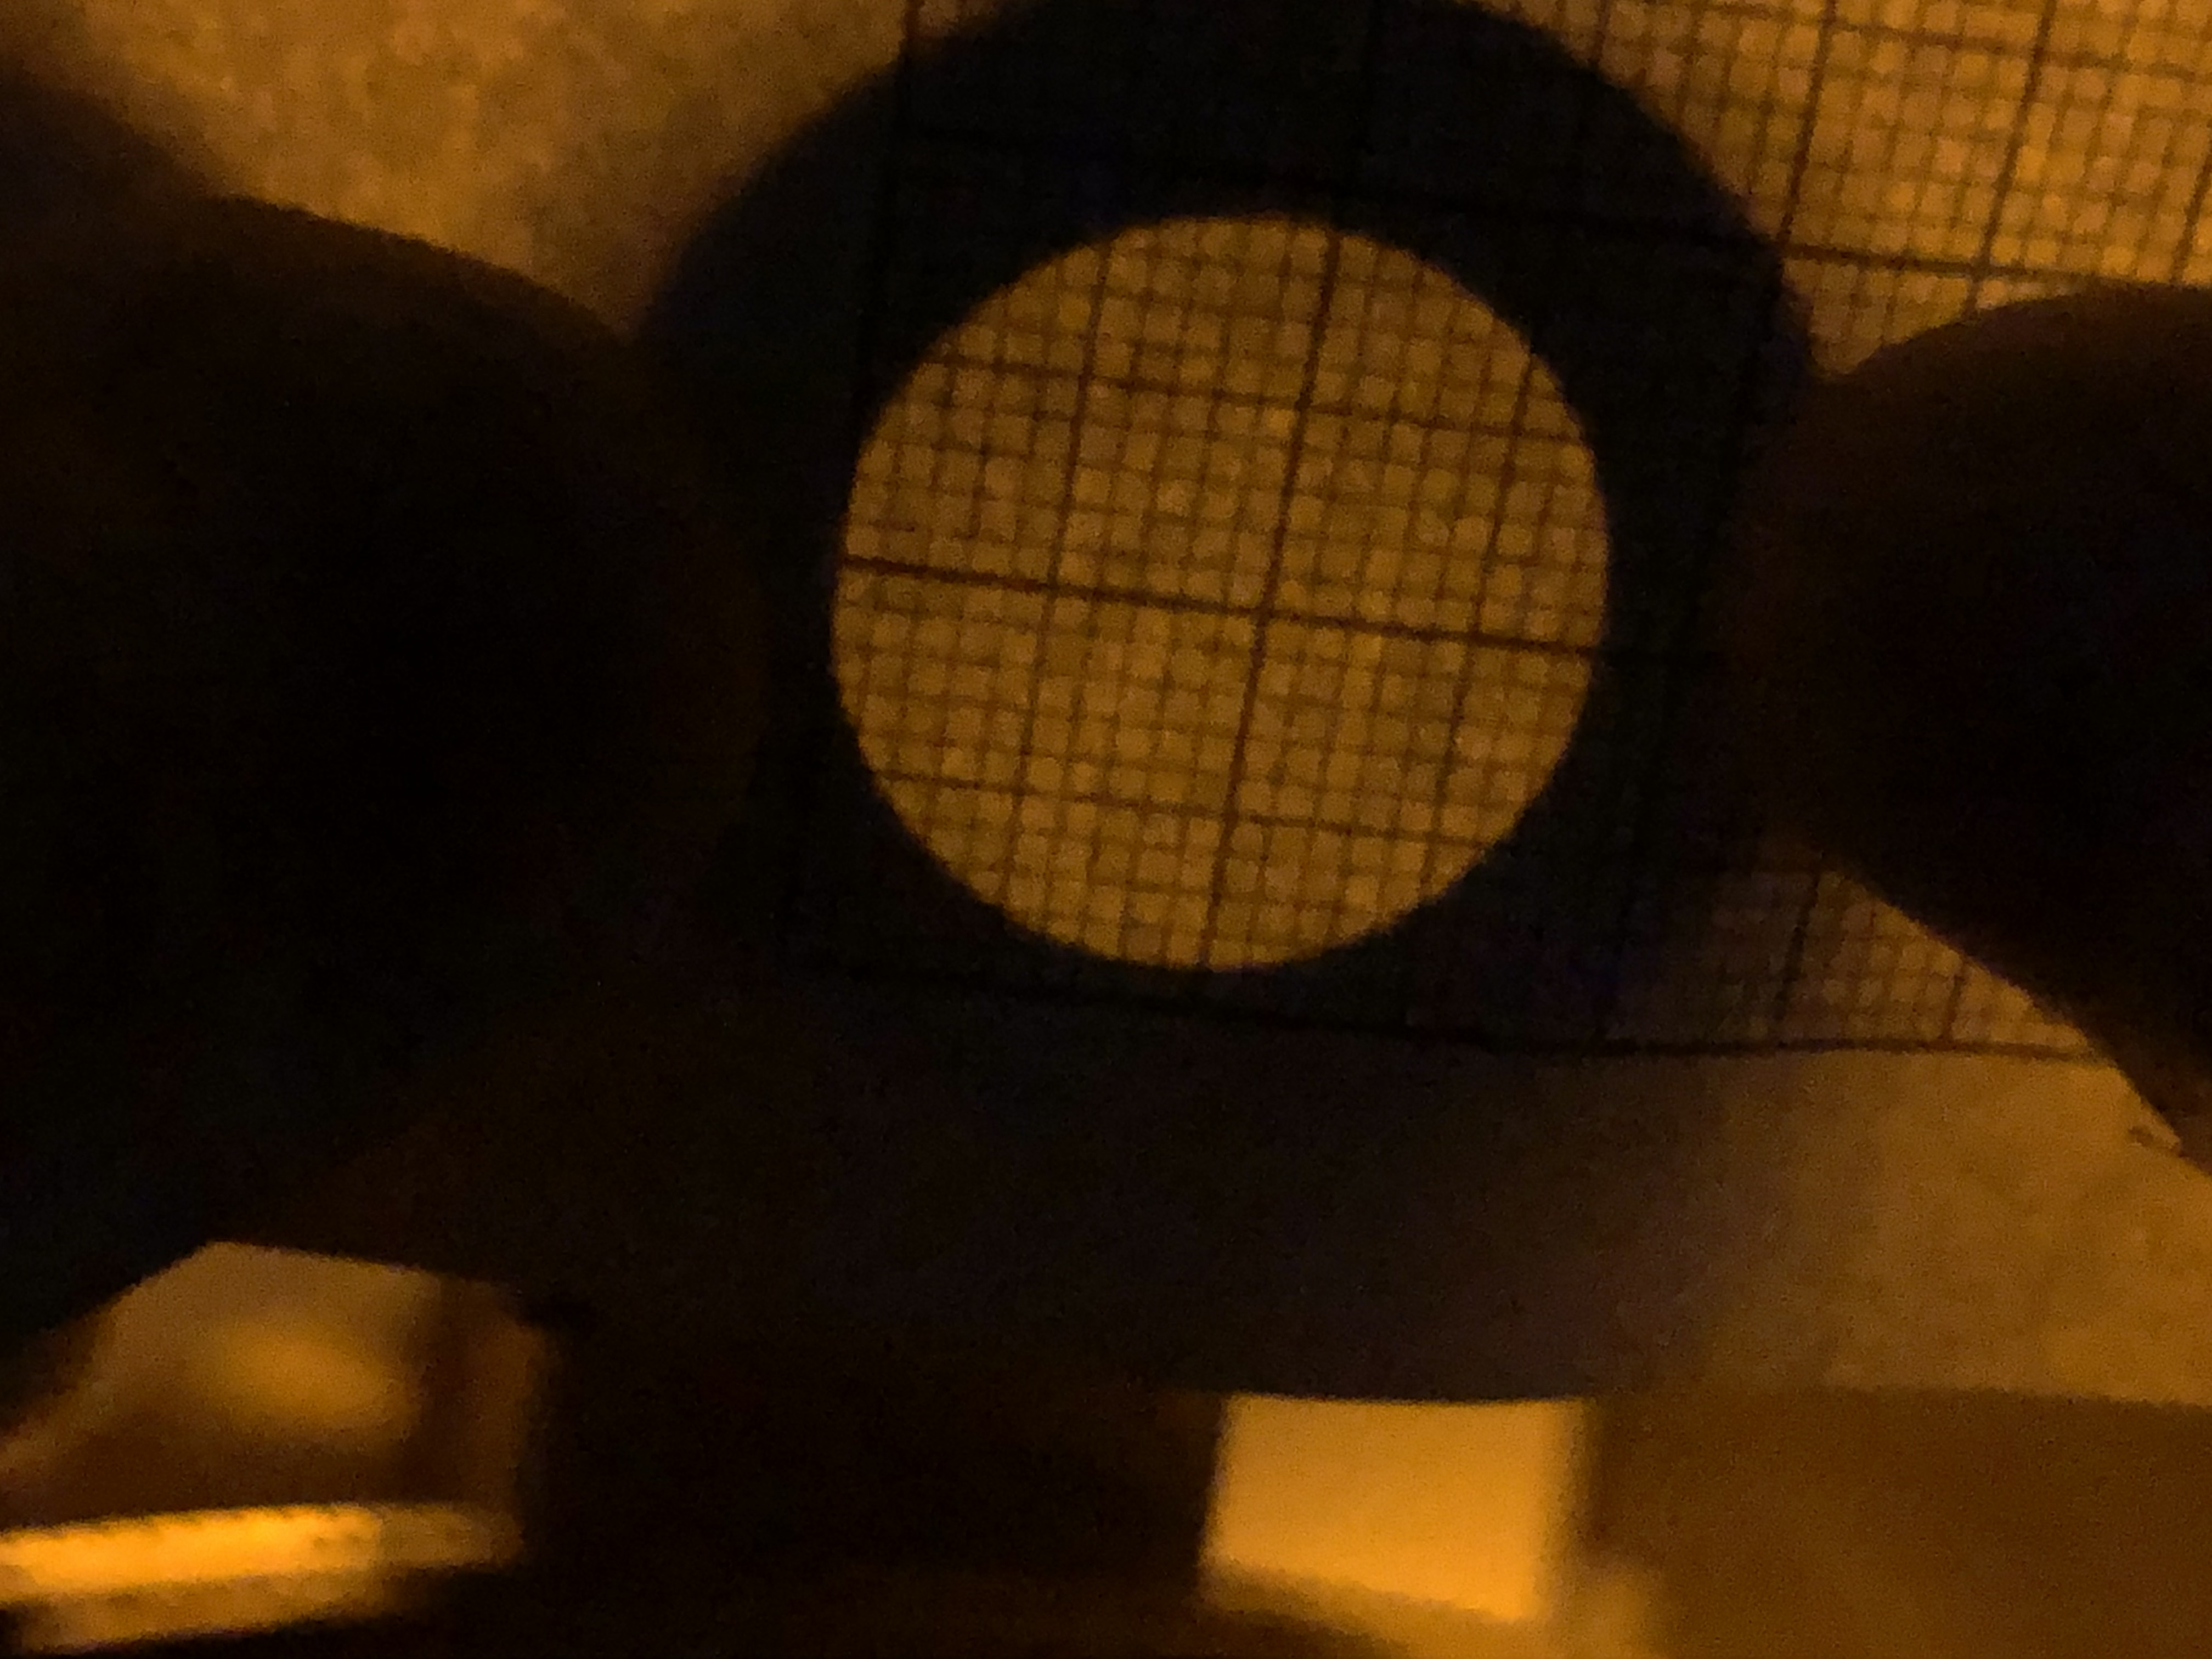
\includegraphics[width=0.5\textwidth]{mmp}
	\end{center}
	\caption{Bestimmung des Durchmessers des Kollimators mithilfe von Millimeterpapier}
	\label{fig:mmp}
\end{figure}

Anhand der oben ersichtlichen Abbildung wird nun der Durchmesser des
Kollimators anhand der Pixelanzahl bestimmt und so anhand des Maßstabs des Millimeterpapiers auf die Größe geschlossen, was einen Durchmesser von

\begin{equation}
	D = \SI{1.809(16)}{cm}
	\label{eq:durchmesser}
\end{equation}

liefert.

\newpage

\subsection{Prisma}

\subsubsection{Brechender Winkel}

Um den brechenden Winkel des Prismas zu bestimmen, wird dieses auf den Sockel
des Spektrometertisches gestellt, sodass die Spitze des Prismas direkt auf die
Lichtquelle zeigt. Dadurch entstehen 2 Lichtpunkte, deren Winkel erneut
mithilfe des Fernrohrs bestimmt werden müssen. Diese Messung wird auch nach
vorsichtigen Verrücken des Prismas mehrmals wiederholt, wodurch folgende Werte
entstehen.

\begin{table}[H]
	\caption{gemessene linke und rechte Winkel des abgelenkten Strahls\\ $\varphi_r \dots$ abgelesener Winkel nach rechts \\ $\varphi_l \dots$ abgelesener Winkel nach links}
	\label{tab:messgamma}
	\centering
	\begin{tabular}{lrr}
\toprule
{} &  $\varphi_r$ / \si{\degree} &  $\varphi_l$ / \si{\degree} \\
\midrule
0 &                        56.7 &                       297.0 \\
1 &                        59.8 &                       300.1 \\
2 &                        54.5 &                       295.3 \\
3 &                        64.5 &                       304.8 \\
4 &                        64.4 &                       304.6 \\
\bottomrule
\end{tabular}

\end{table}


\subsubsection{Brechungsindex}

Um den Brechungsindex zu bestimmen, wird das Prisma, wie in
\autoref{fig:prisma_st} sichtbar, mit der matten Seite in den Strahlengang
gestellt, wodurch sich das weiße Licht der Lampe in seine Spektralen
Bestandteile zerlegt, wie in \autoref{fig:farben} sichtbar.

\vspace{2mm}

\begin{minipage}{\textwidth}
	\begin{minipage}[t]{0.35\textwidth}
		\centering
		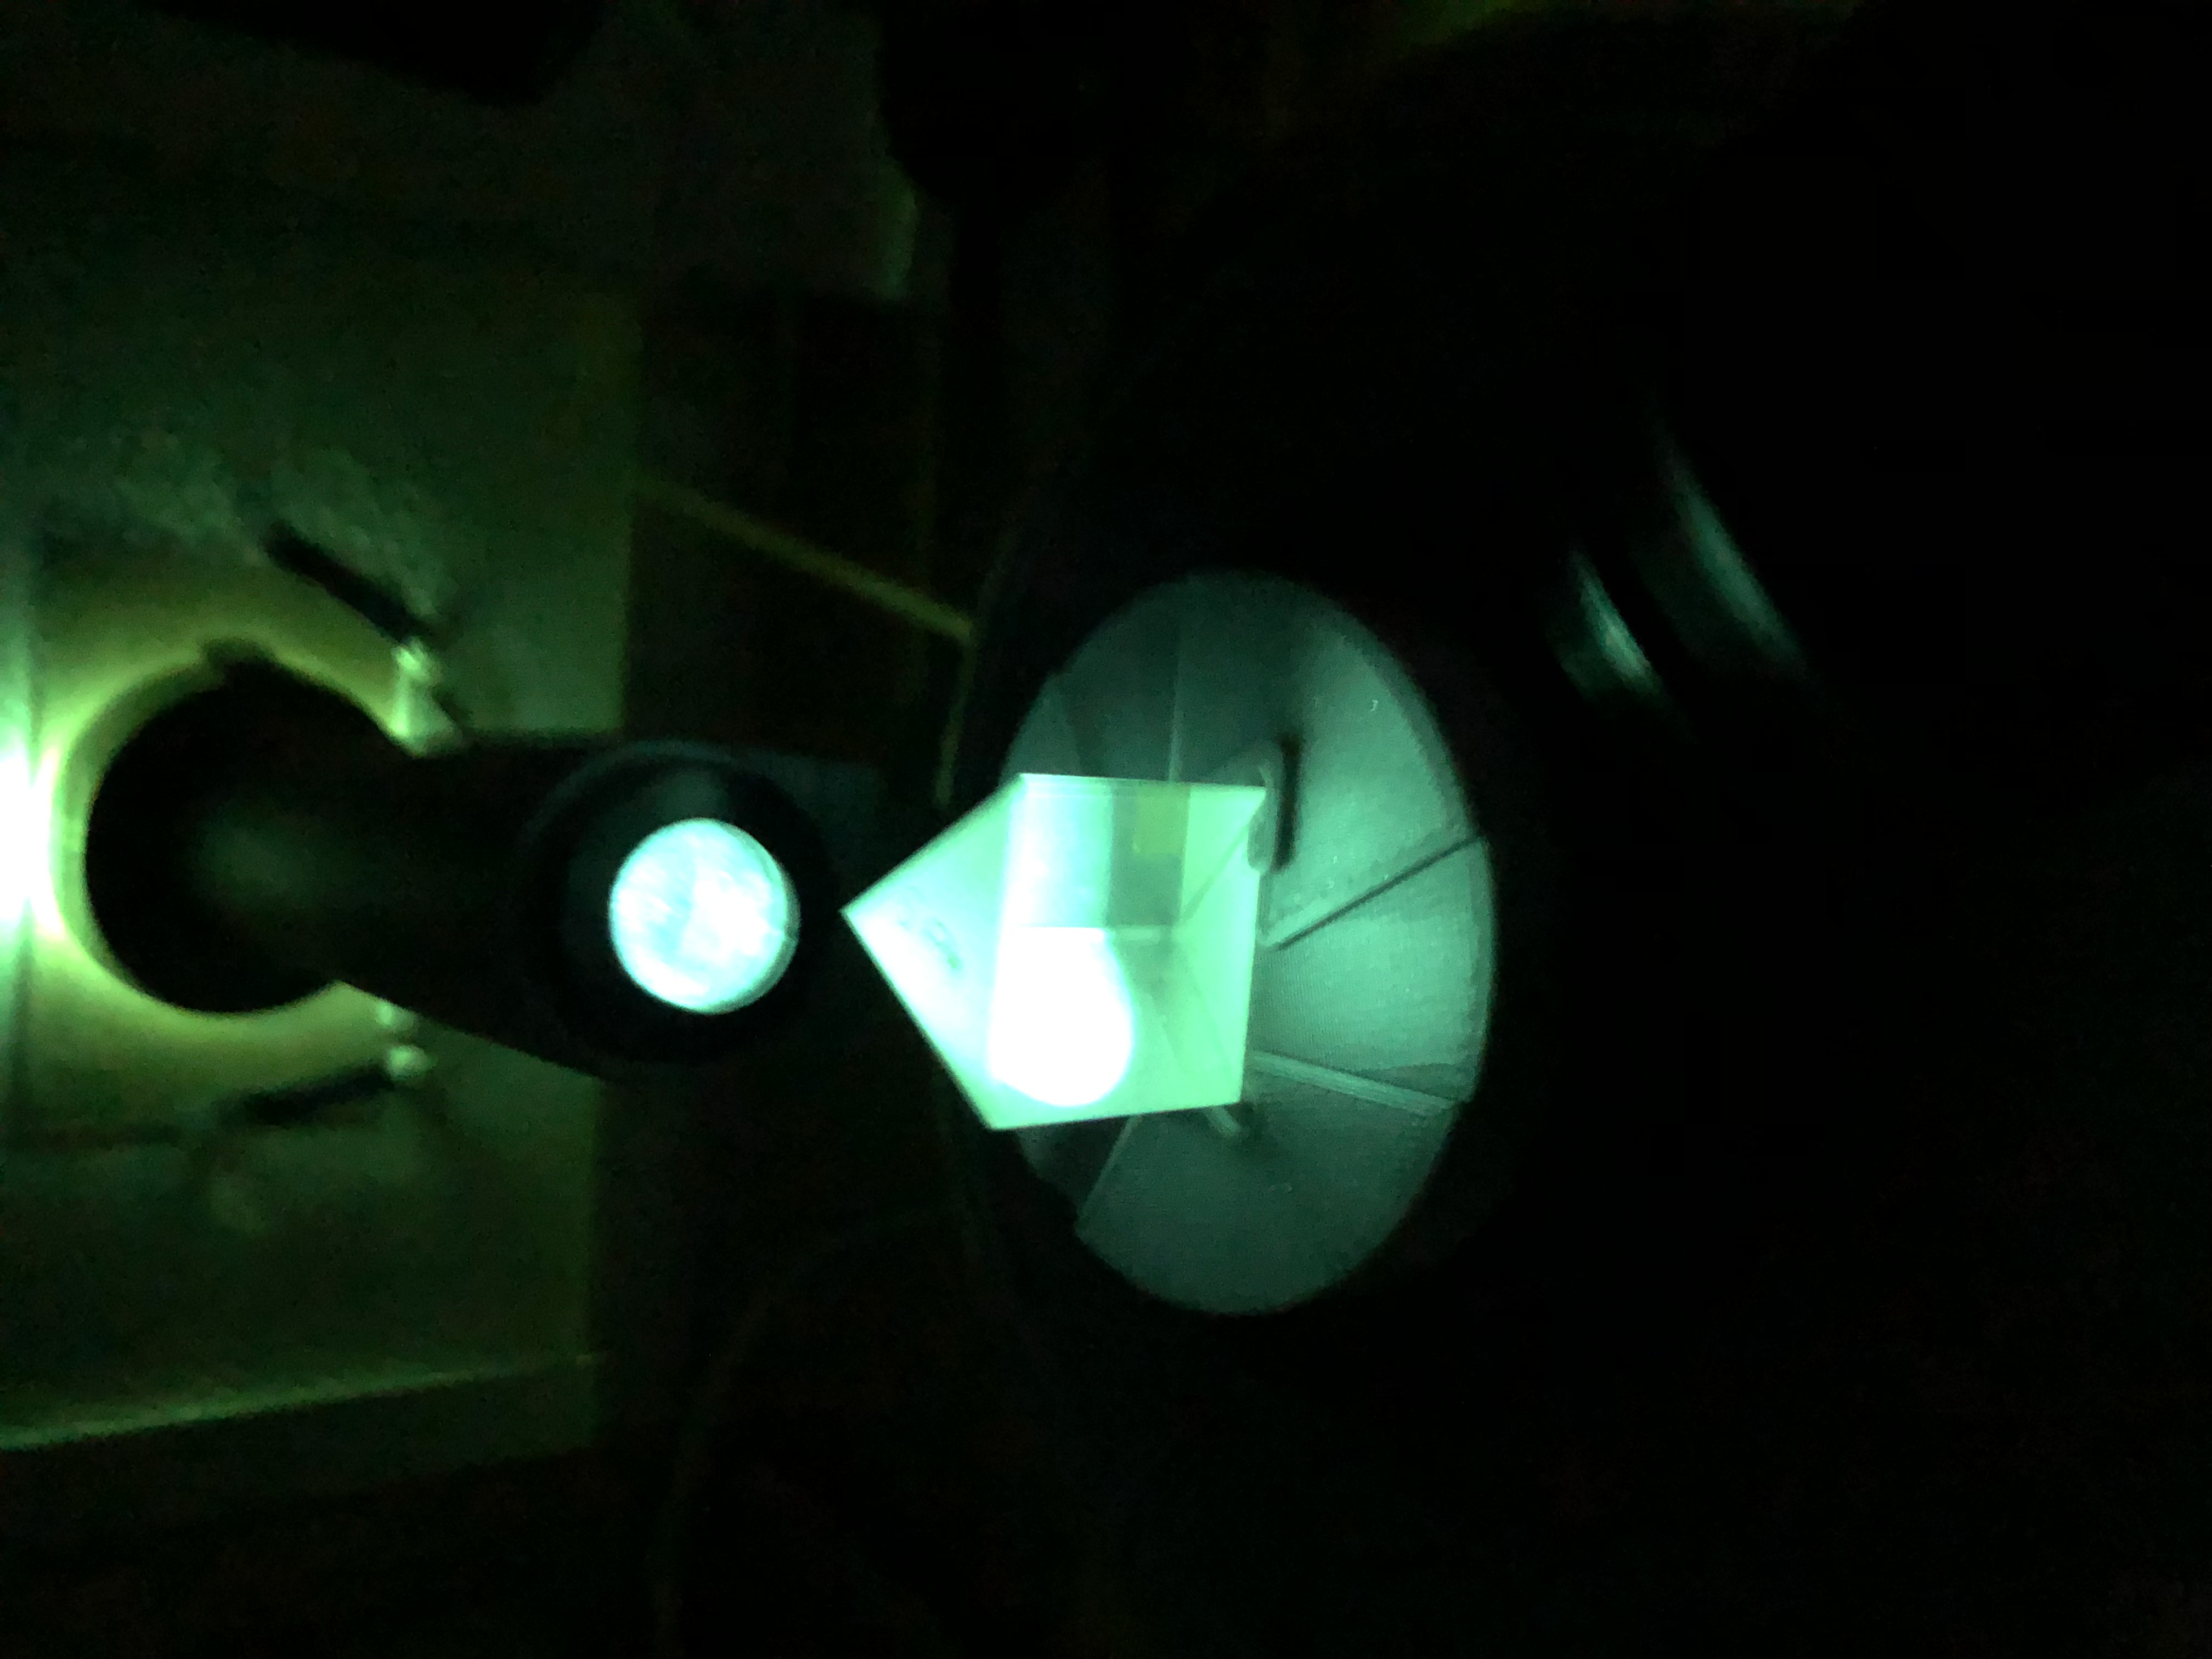
\includegraphics[angle=-90,width=\textwidth]{prisma_st}
		\captionbelowof{figure}{Prisma in Strahlengang}
		\label{fig:prisma_st}
	\end{minipage}
	\vspace{2mm}
	\begin{minipage}[t]{0.63\textwidth}
		\centering
		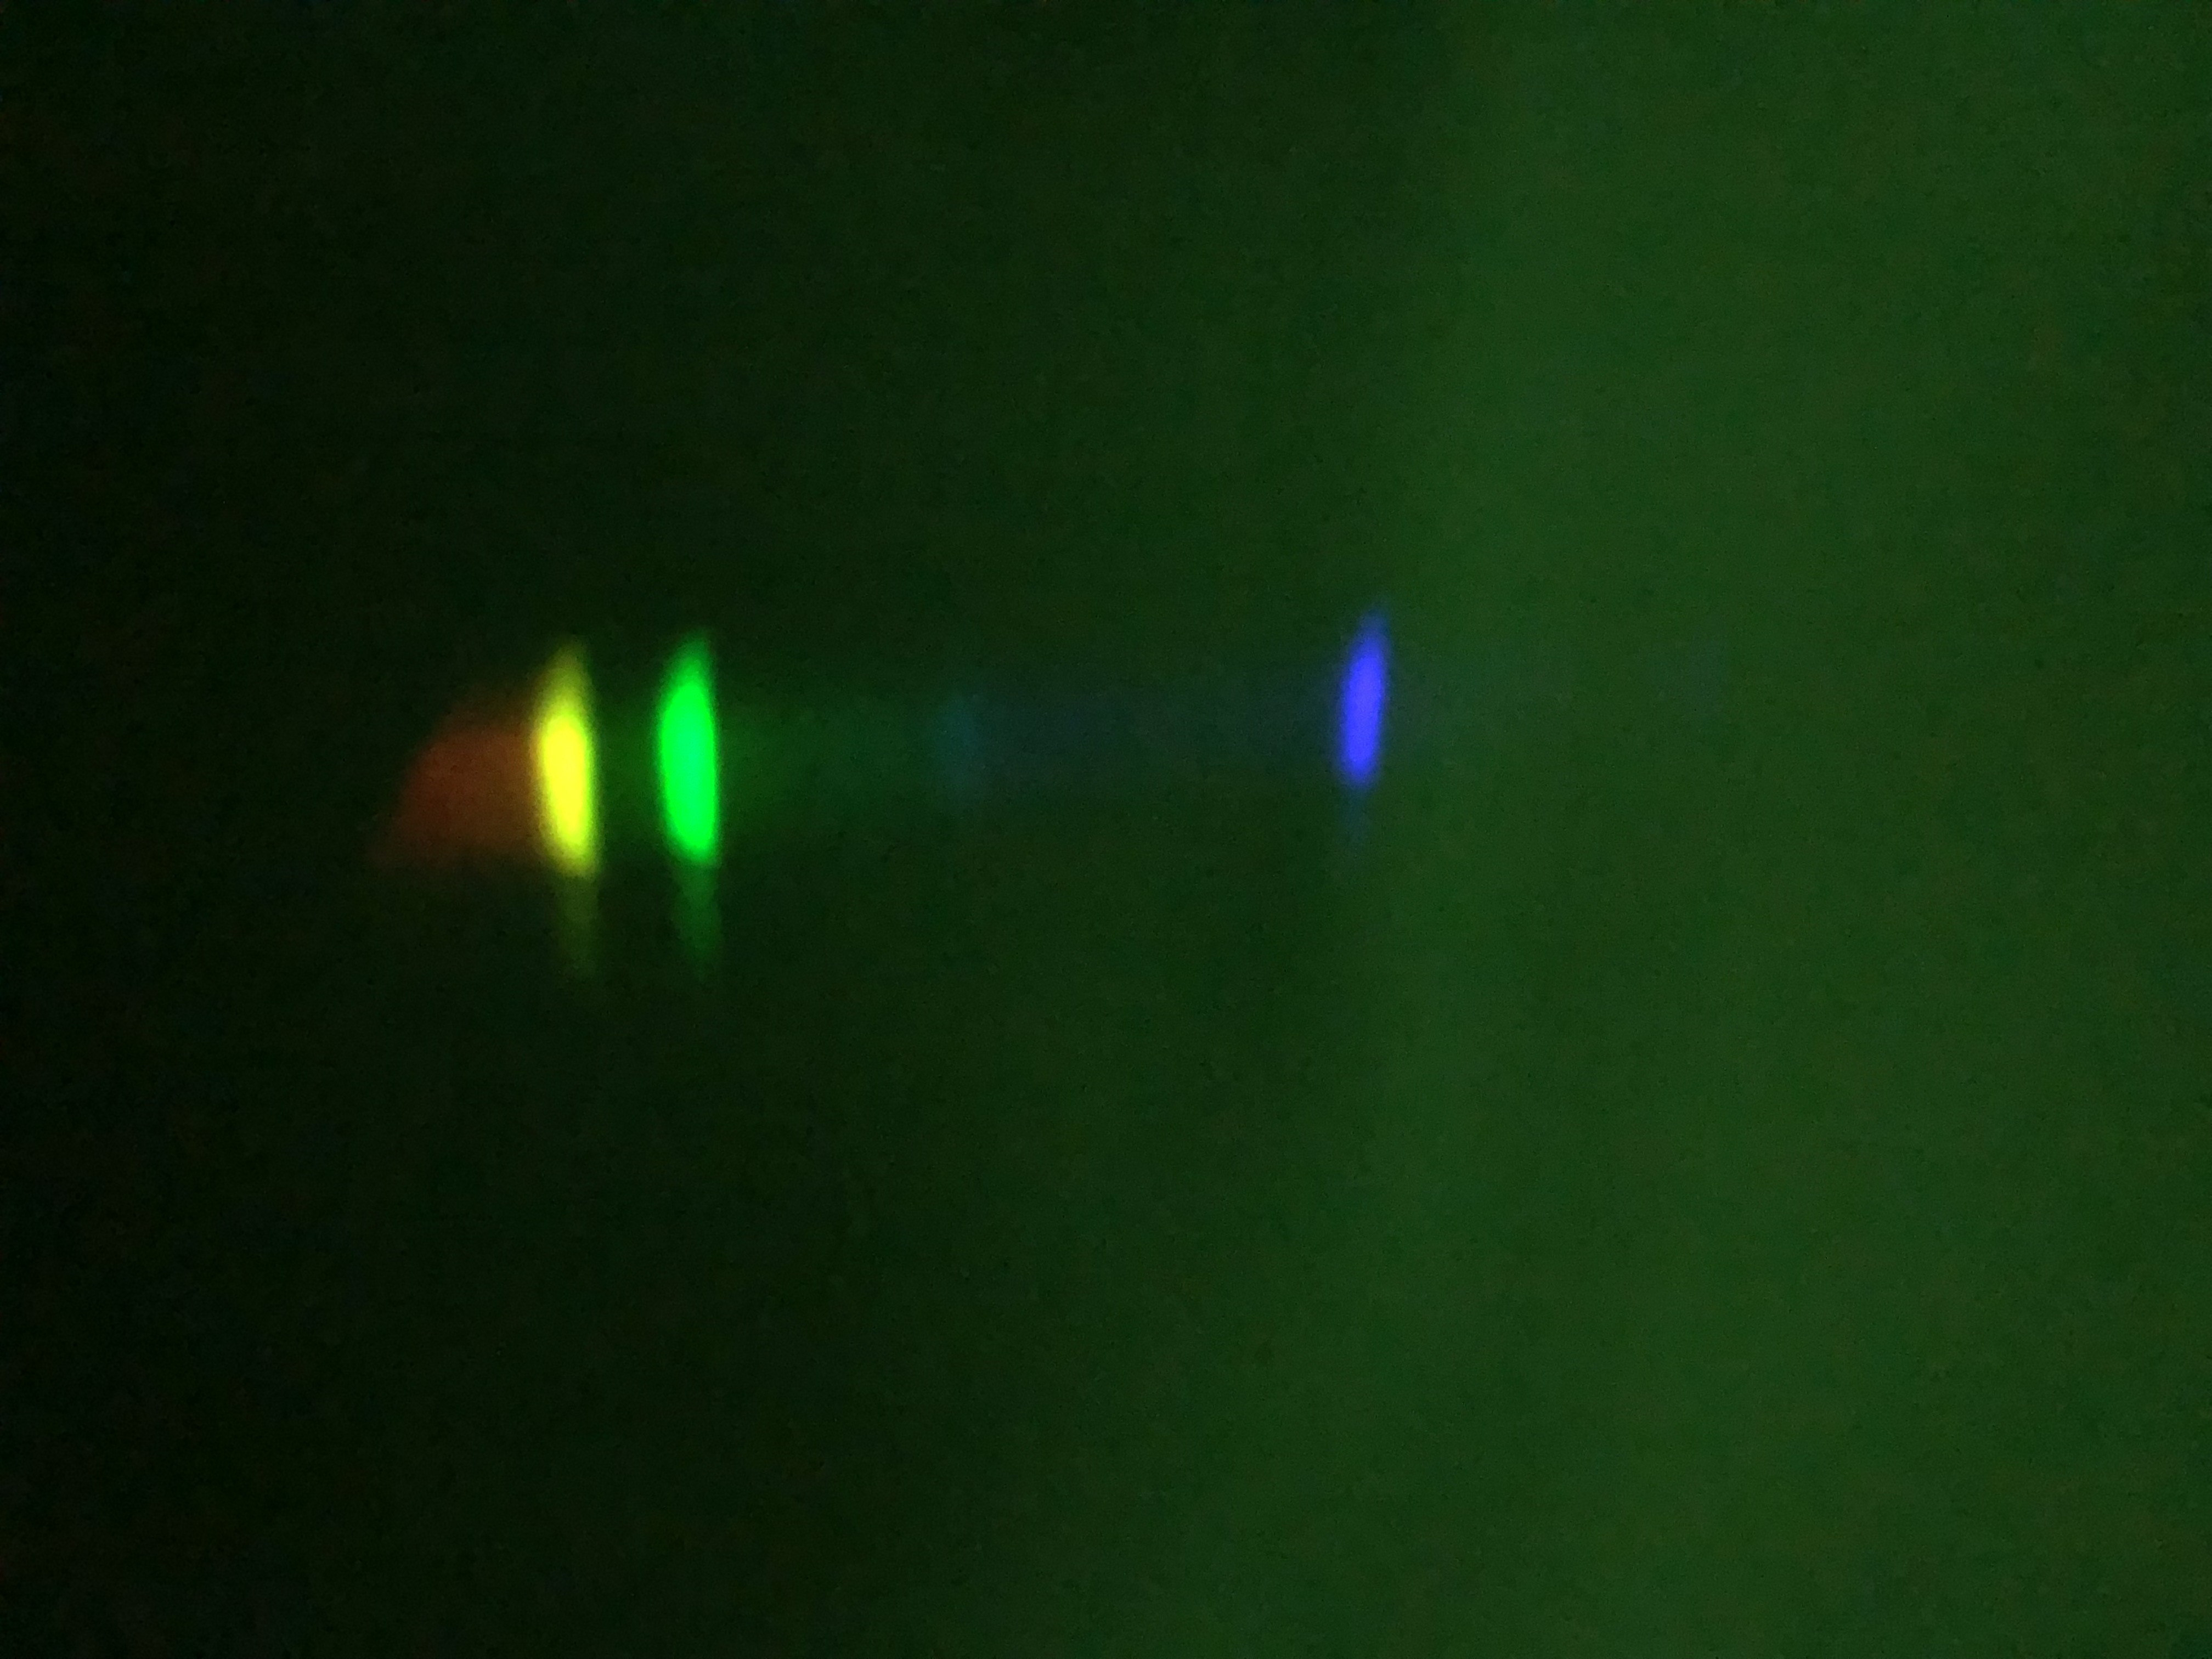
\includegraphics[width=\textwidth]{farben}
		\captionof{figure}{Spektrale Aufteilung des weißen Lichts}
		\label{fig:farben}
	\end{minipage}
	\vspace{1em}
\end{minipage}

Nun wird das Prisma vorsichtig gedreht, sodass der größtmögliche
Ablenkungswinkel erreicht werden kann. Dies kann durch Blick durch das Fernrohr
noch genauer bestimmt werden. Bei der so ermittelten Position des Prismas
werden nun die Winkel bei den entsprechenden Farben notiert, was in folgender
Tabelle sichtbar ist. Dieser Vorgang wird sowohl für die linke als auch für die
rechte Seite wiederholt.

\begin{table}[H]
	\caption{gemessene linke und rechte Winkel des zerlegten Strahls bei der entsprechenden Wellenlänge\\ $\varphi_r \dots$ abgelesener Winkel nach rechts \\ $\varphi_l \dots$ abgelesener Winkel nach links}
	\centering
	\label{tab:messalle}
	\begin{tabular}{lrr}
	\toprule
	{}        & $\varphi_r$ / \si{\degree} & $\varphi_l$ / \si{\degree} \\
	\midrule
	Dunkelrot & 64.6                       & 295.4                      \\
	Rot       & 65.1                       & 294.6                      \\
	Gelb1     & 65.9                       & 294.0                      \\
	Gelb2     & 66.0                       & 293.8                      \\
	Grün      & 66.8                       & 293.1                      \\
	Blaugrün  & 68.5                       & 291.4                      \\
	Indigo    & 71.4                       & 287.6                      \\
	Violett1  & 73.9                       & 286.3                      \\
	Violett2  & 74.2                       & 286.0                      \\
	\bottomrule
\end{tabular}

\end{table}

Um den Fehler der durch das Einrichten des Prismas entsteht möglichst gering zu halten, wird die Messung noch weitere 5 mal wiederholt.

Jedoch wurden hier nur die Winkel der am weitesten außen liegenden Farben, also Dunkelrot und Violett, notiert, wodurch folgende Tabelle entsteht.

\begin{table}[H]
	\caption{gemessene linke und rechte Winkel des zerlegten Strahls bei den außenliegenden Wellenlängen\\ $\varphi_r \dots$ abgelesener Winkel nach rechts bei der entsprechenden Farbe\\ $\varphi_l \dots$ abgelesener Winkel nach links bei der entsprechenden Farbe}
	\centering
	\label{tab:messextrem}
	\begin{tabular}{lrrrr}
\toprule
{} &  $\varphi_{\text{Violett}_r}$ / \si{\degree} &  $\varphi_{\text{Violett}_l}$ / \si{\degree} &  $\varphi_{\text{Dunkelrot}_r}$ / \si{\degree} &  $\varphi_{\text{Dunkelrot}_l}$ / \si{\degree} \\
\midrule
0 &                                         74.2 &                                        286.0 &                                           64.6 &                                          295.4 \\
1 &                                         73.9 &                                        285.9 &                                           64.2 &                                          295.4 \\
2 &                                         75.8 &                                        286.0 &                                           64.4 &                                          295.3 \\
3 &                                         74.1 &                                        286.0 &                                           64.4 &                                          295.3 \\
4 &                                         74.8 &                                        285.1 &                                           64.9 &                                          295.5 \\
5 &                                         74.0 &                                        285.8 &                                           64.4 &                                          295.6 \\
\bottomrule
\end{tabular}

\end{table}

Die Mittelwerte sind:


\begin{align*}
	\varphi_{\text{Dunkelrot}} & = \SI{64.53(5)}{\degree}  \\
	\varphi_{\text{Violett}}   & = \SI{74.33(17)}{\degree}
\end{align*}


Weil die dunkelrote Linie sehr schwer eindeutig zu bestimmen ist, empfiehlt es sich dabei die Intensität durch Variation der Spaltbreite anzupassen und die orangen Linien mithilfe einer Karte abzudecken um so die roten Linien besser identifizieren zu können, ohne dem Auge dabei zu große Qualen auszusetzen. Dieses einschieben der Karte ist in folgender \autoref{fig:abdecken} sichtbar.

\begin{figure}[H]
	\begin{center}
		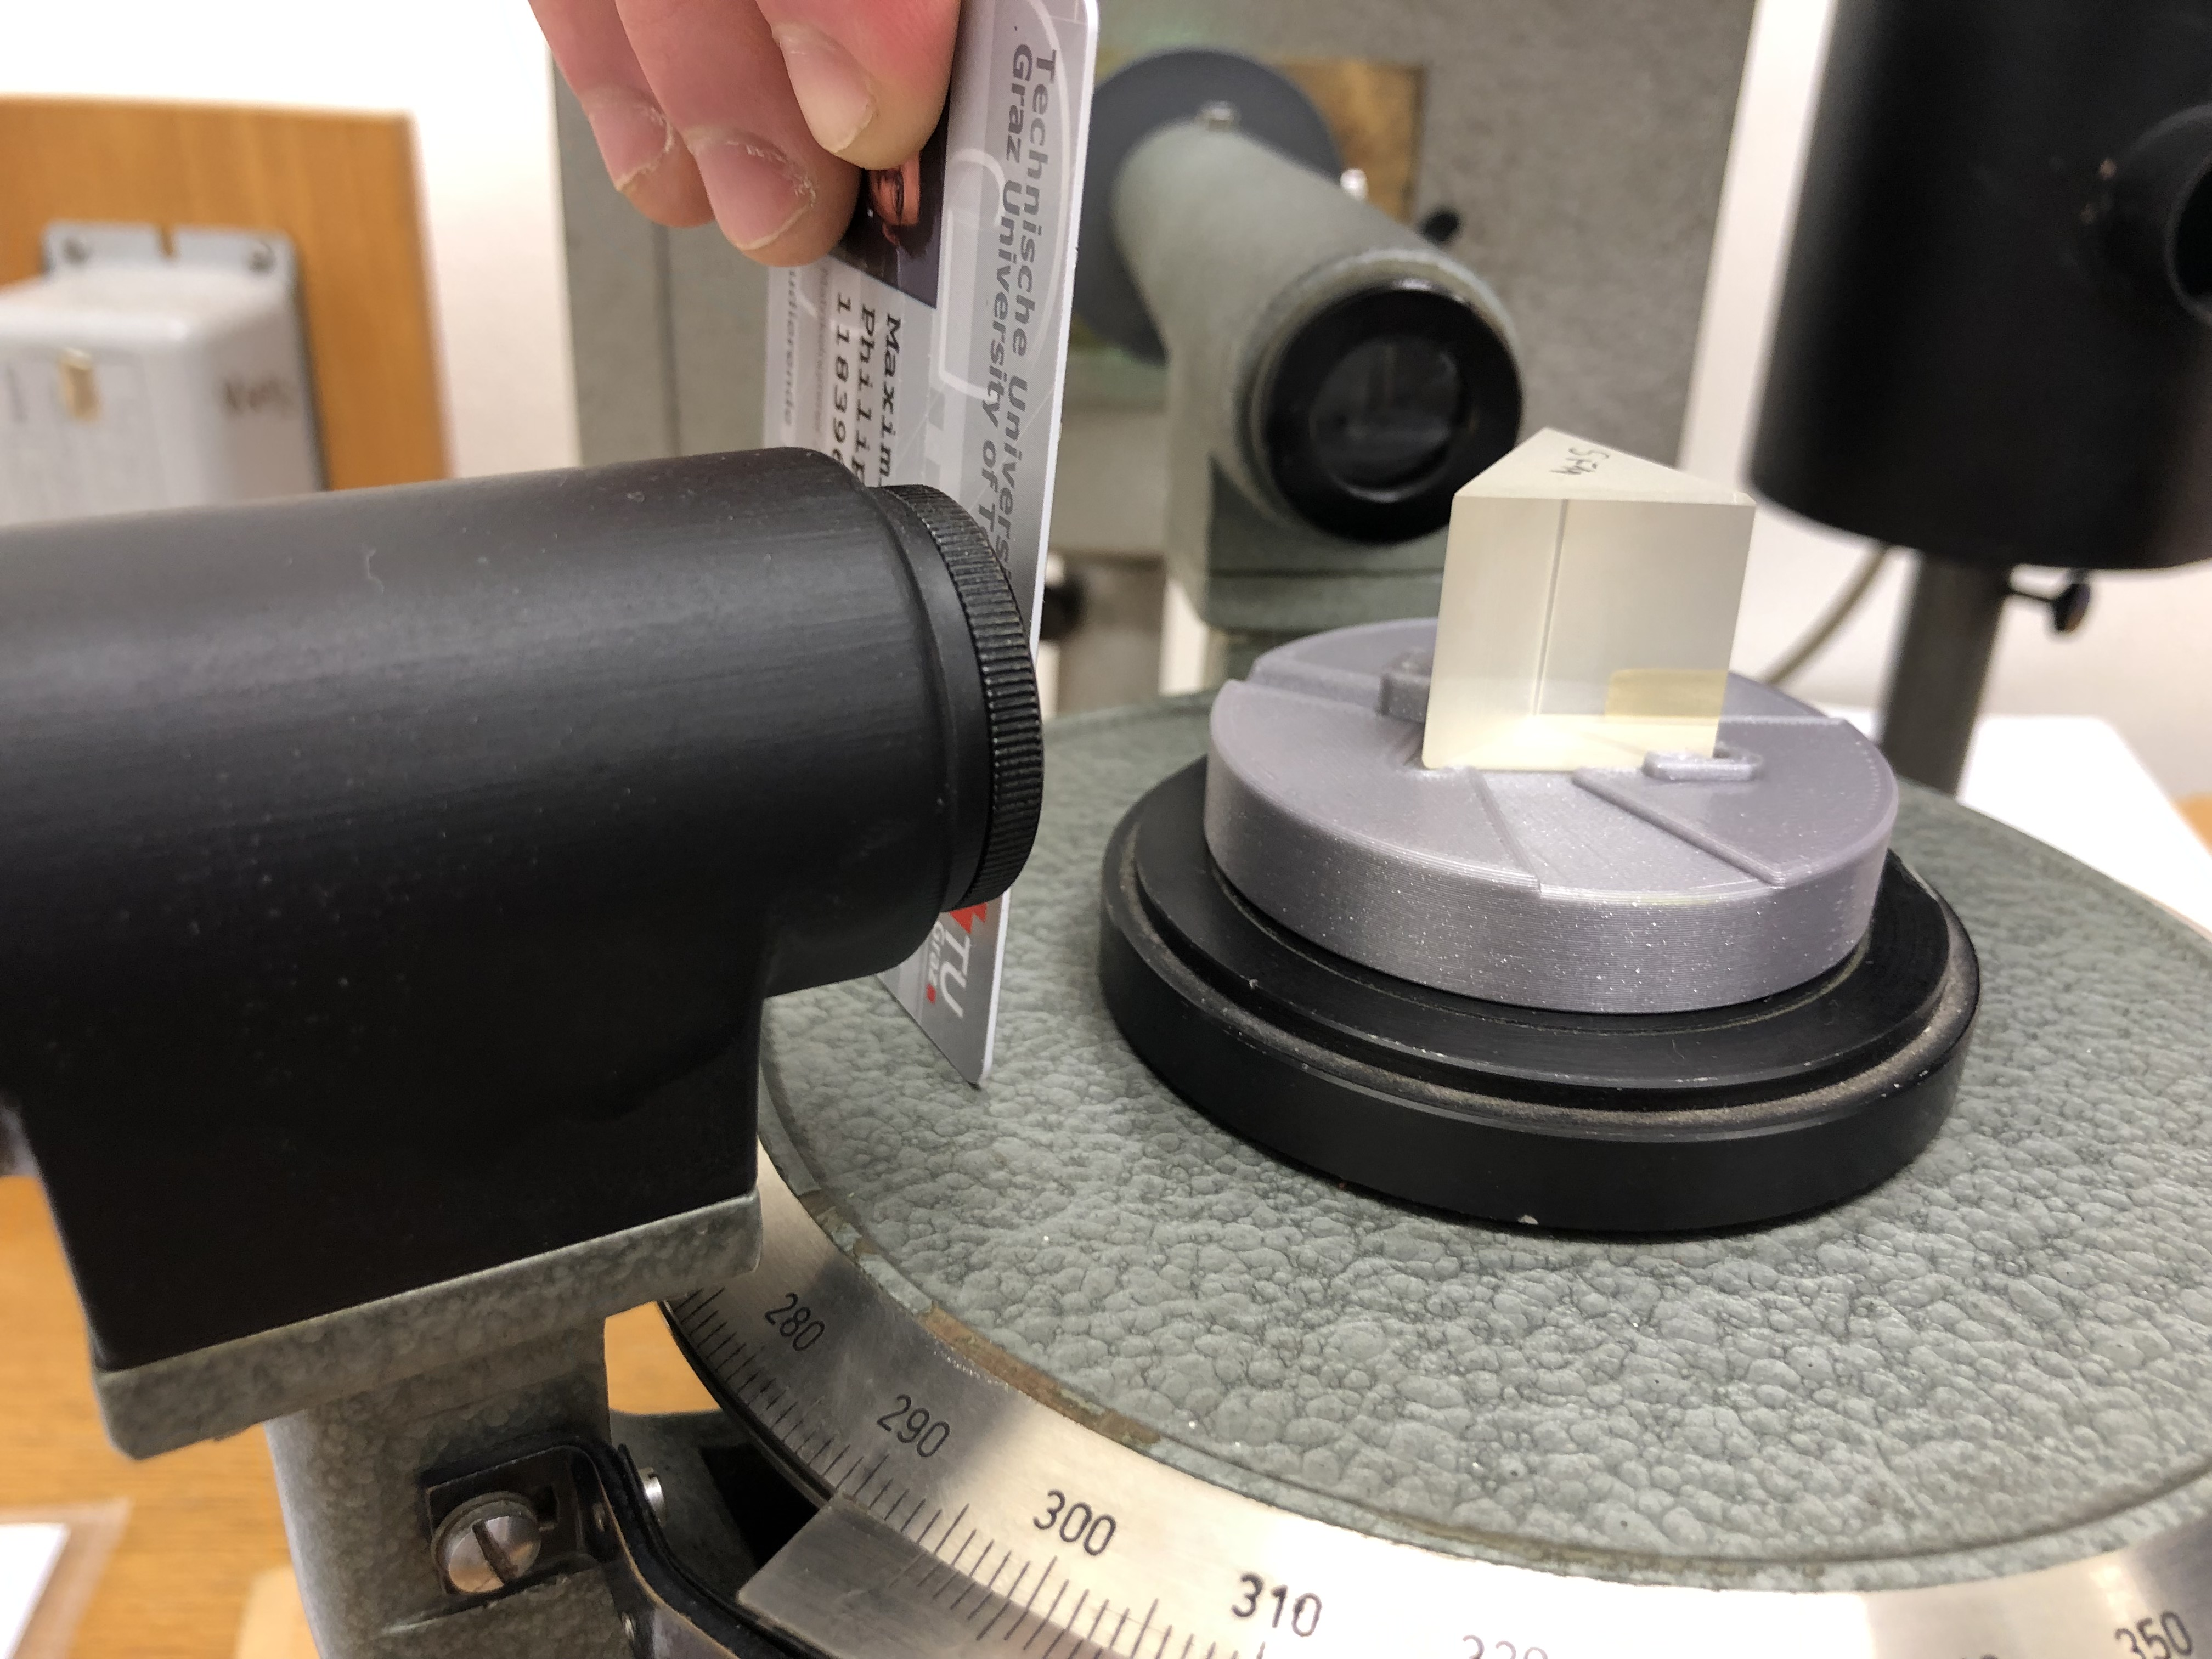
\includegraphics[width=0.5\textwidth]{abdecken}
	\end{center}
	\caption{Einschieben einer Karte um die intensiveren Spektren auszublenden}
	\label{fig:abdecken}
\end{figure}


\subsubsection{Auflösungsvermögen}

Um des Auslösevermögen bestimmen zu können, muss nur der Durchmesser des
Kollimators gemessen werden. Da es sich dabei um den selben wie zuvor handelt
wird hier auch der, zuvor mithilfe von Millimeterpapier bestimmte, Wert von
\SI{1.809(16)}{cm} übernommen.



\section{Auswertung}

\noindent Um zu sehen wie sich die Unsicherheit der Messungen bis in die
Ergebnisse fortpflanzt, ist \autoref{eq:Unsicherheitsfortpflanzung} verwendet
worden. Die Grundlagen dieser Gleichung stammen von den Powerpointfolien von
GUM.\cite{WolfgangKessel2004} Die Verallgemeinerung ist von Wikipedia entnommen
worden \cite{2020Fehler}. Für die Auswertung ist die Progammiersprache Python
im speziellen das Packet \verb#scipy#, zur Hilfe genommen worden.

\begin{equation}
	\label{eq:Unsicherheitsfortpflanzung}
	V_y = J(x) \cdot V_x \cdot J^{T}(x)
\end{equation}

\noindent Wobei $V_y$ und $V_x$ die Kovarianzmatrizen von den Vektoren $\bm{y}$ und $\bm{x}$ sind.
$\bm{x}$ ist der Vektor der Eingangsvariablen und $\bm{y}$ ist der Vektor der Ausgangsvariablen.
$J$ ist die Jakobimatrix der vektorwertigen Funktion $\bm{y} = \vec{F}(\bm{x})$.
So lassen sich die Komponenten der Matrix relativ einfach anschreiben $J_{ij}(x) = \frac{\partial{y_i}}{\partial{x_j}}(x)$.
Damit man die Unsicherheit der einzelnen Variablen $y_i$ bekommt, muss nur die Quadratwurzel des i-ten Diagonalelementes der
$\bm{y}$-Kovarianzmatrix genommen werden $u_i= \sqrt{\mathrm{diag}(V_y)_i}$.
Da in diesem Experiment meistens nur skalare Funktionen untersucht werden, vereinfacht
sich die \autoref{eq:Unsicherheitsfortpflanzung} dramatisch und die Unsicherheit
der Variable $y$ lässt sich einfach so berechnen:

\begin{equation}
	\label{eq:graduncentainty}
	u_y = \sqrt{\mathrm{grad} y^T \cdot V_x \cdot \mathrm{grad} y}
\end{equation}

Für die erhaltenen Werte wurde von einer Normalverteilung ausgegangen, weshalb
der jeweilige student t Korrekturfaktor für ein 3 $\sigma$ Konfidenzintervall
verwendet werden muss.

Es wurde jedes mal der doppelte Winkel gemessen. Um dann auf die gesuchten Winkel zu kommen wurden diese so berechnet

\begin{equation}
	\phi = (\phi_r + 360 - \phi_l) / 2
	\label{eq:messwertzuwinkel}
\end{equation}
\subsection{Gitter}

\subsubsection{Gitterkonstante}

Der Winkel wurde mit folgender Gleichung berechnet. Daraus wurde dann $g$ bestimmt, indem \autoref{eq:gitterkonstante} auf $g$ umgeformt wird.
\begin{equation}
	g = 2* (5880.95 + 5895.92) / (2 * sin(pi * phi / 180) * 10 ** 7)
	% \label{eq:}
\end{equation}

So kommt man auf folgende Werte:

\begin{table}[H]
	\caption{erhaltene Gitterkonstanten und Winkel zweite Ordnung \\ $\varphi \dots$ erhaltener Winkel 2. Ordnung \\ $g \dots$ erhaltene Gitterkonstante \\ $\Delta \dots $ entsprechende Unsicherheit}
	\centering
	\label{tab:wertgitter}
	\begin{tabular}{lrrrr}
\toprule
{} &  $\varphi$ / \si{\degree} &  $\Delta \varphi$ / \si{\degree} &  $g$ / mm &  $\Delta g$ / mm \\
\midrule
0 &                     42.40 &                              0.2 &  0.001747 &         0.000007 \\
1 &                     42.30 &                              0.2 &  0.001750 &         0.000007 \\
2 &                     42.25 &                              0.2 &  0.001752 &         0.000007 \\
3 &                     42.35 &                              0.2 &  0.001748 &         0.000007 \\
4 &                     42.35 &                              0.2 &  0.001748 &         0.000007 \\
5 &                     42.35 &                              0.2 &  0.001748 &         0.000007 \\
\bottomrule
\end{tabular}

\end{table}

Daraus wurde der Mittelwert bestimmt, was folgenden Wert ergibt:

\begin{equation}
	\bar{g} = \SI{0.0017488(7)}{\mm}
	\label{eq:gbar}
\end{equation}

Da $g$ nun bekannt ist, kann auch auf die Verdrehung des Gitters
zurückgeschlossen werden, indem die echte Gitterkonstante durch den erhalten Wert
dividieren und davon der arccos genommen wird, was im folgenden sichtbar ist.

\begin{equation}
	\bar{\varphi_0} = \arccos(\frac{g'}{g}) = \SI{4.6(3)}{\degree}
	\label{eq:initialangle}
\end{equation}

Dadurch erhält man eine Verschiebung von ungefähr
\SI{4.6(3)}{\degree} zur perfekten frontal Einstellung. Diese Information kann
verwendet werden um das Gitter perfekt orthogonal einzurichten
indem die maximale Gitterkonstante $g$ gefunden wird.

\subsubsection{Wellenlänge}

Für die folgenden Berechnungen muss $z = 2$ angenommen werden, da immer die zweite Ordnung bestimmt wurde.

Nun wird der Mittelwert von $g$ in verwendet, indem \autoref{eq:auflvermgitter} auf $\lambda$ umgeformt wird, was folgende Werte liefert.
% \begin{equation}
%   \lambda = \frac{g}{2}(\sin{\varphi}+\sin{\varphi_0})
%   \label{eq:}
% \end{equation}

\begin{table}[H]
	\caption{Berechnete Wellenlängen anhand der Gitterkonstanten und der gemessenen Winkel zweite Ordnung \\ $\varphi \dots$ erhaltener Winkel 2. Ordnung \\ $\lambda \dots$ erhaltene Wellenlänge \\ $\Delta \dots $ entsprechende Unsicherheit}
	\centering
	\label{tab:wertwellenlange}
	\begin{tabular}{lrrrr}
	\toprule
	{}      & $\varphi$ / \si{\degree} & $\Delta \varphi$ / \si{\degree} & $\lambda$ / \si{\nm} & $\Delta \lambda$ / \si{\nm} \\
	\midrule
	Violett & 27.60                    & 0.2                             & 405                  & 3                           \\
	Blau    & 29.90                    & 0.2                             & 436                  & 3                           \\
	Türkis1 & 34.25                    & 0.2                             & 492                  & 3                           \\
	Türkis2 & 34.65                    & 0.2                             & 497                  & 3                           \\
	Grün    & 38.65                    & 0.2                             & 546                  & 3                           \\
	Orange1 & 41.30                    & 0.2                             & 577                  & 3                           \\
	Orange2 & 41.55                    & 0.2                             & 580                  & 3                           \\
	Rot1    & 44.05                    & 0.2                             & 608                  & 3                           \\
	Rot2    & 45.55                    & 0.2                             & 624                  & 3                           \\
	\bottomrule
\end{tabular}

\end{table}

\subsubsection{Auflösungsvermögen}
Auch hier wurde wieder $z = 2$ angenommen, da die zweite Ordnung gemessen wurde. Der bestimmte Mittelwert von der Gitterkonstante $g$ und Dicke des Rohrs wurden mit \autoref{eq:auflvermgitter} verwendet um folgende Werte zu erhalten.

\begin{equation}
	\frac{\lambda}{\Delta \lambda} = z \frac{D}{g} = 2 \frac{\num{18.09(16)}}{\num{0.0017488(7)}} = \num{2.069(18)e+04}
	\label{eq:auflosunggitter}
\end{equation}

\newpage

\subsection{Prisma}

\subsubsection{Brechender Winkel}

Auch hier wurden wieder \autoref{eq:messwertzuwinkel} und \autoref{eq:gamma} verwendet, um auf folgende Werte zu kommen.

\begin{table}[H]
	\caption{bestimmte Werte für den brechenden Winkel \\ $\gamma \dots$ erhaltener Wer für den brechenden Winkel \\ $\Delta \dots $ entsprechende Unsicherheit}
	\centering
	\label{tab:brechenderwinkel}
	\begin{tabular}{lrr}
\toprule
{} &  $\gamma$ / \si{\degree} &  $\Delta \gamma$ / \si{\degree} \\
\midrule
0 &                    59.85 &                             0.2 \\
1 &                    59.85 &                             0.2 \\
2 &                    59.60 &                             0.2 \\
3 &                    59.85 &                             0.2 \\
4 &                    59.90 &                             0.2 \\
\bottomrule
\end{tabular}

\end{table}

Daraus wird wieder der Mittelwert gebildet was folgenden Wert ergibt.

\begin{equation}
	\gamma = \SI{59.81(5)}{\degree}
	\label{eq:gammabar_wert}
\end{equation}

\subsubsection{Brechungsindex}

Der Winkel wurde mit \autoref{eq:messwertzuwinkel} berechnet und dann mittels
$\gamma$ in \autoref{eq:brechzahl} verwendet, um folgende Werte zu erhalten.

\begin{table}[H]
	\caption{erhaltene Brechzahlen \\ $\delta \dots$ gemessener Winkel \\
		$\lambda \dots$ gegebene Wellenlänge \\ $n \dots$ erhaltene Brechzahl \\
		$n_{theo} \dots$ verglichene Literaturwerte \cite{brechzahl} \\ $\Delta \dots$
		entsprechende Unsicherheit}
	\centering
	\label{tab:wertbrechzahl}
	\begin{tabular}{lrrrrrr}
	\toprule
	{} & $\delta$ / \si{\degree} & $\Delta \delta$ / \si{\degree} & $\lambda$ / \si{\um} & $n$ / 1 & $\Delta n$ / 1 & $n_{theo}$ / 1 \\
	\midrule
	0  & 64.53                   & 0.05                           & 0.6908               & 1.7738  & 0.0011         & 1.7726  \\
	1  & 65.25                   & 0.2                            & 0.6234               & 1.7796  & 0.0017         & 1.7798  \\
	2  & 65.95                   & 0.2                            & 0.5791               & 1.7852  & 0.0016         & 1.7860  \\
	3  & 66.1                    & 0.2                            & 0.5770               & 1.7864  & 0.0016         & 1.7864  \\
	4  & 66.85                   & 0.2                            & 0.5461               & 1.7924  & 0.0016         & 1.7919  \\
	5  & 68.55                   & 0.2                            & 0.4916               & 1.8055  & 0.0016         & 1.8048  \\
	6  & 71.9                    & 0.2                            & 0.4358               & 1.8304  & 0.0015         & 1.8252  \\
	7  & 73.8                    & 0.2                            & 0.4078               & 1.8436  & 0.0014         & 1.8401  \\
	8  & 74.33                   & 0.17                           & 0.4045               & 1.8451  & 0.0013         & 1.8422  \\
	\bottomrule
\end{tabular}

\end{table}

Fittet man nun die erhaltenen Werte an die ``Sellmeier - Kurve``, bekommt man folgende \autoref{fig:dispersionkurve}:


\begin{figure}[H]
	\begin{center}
		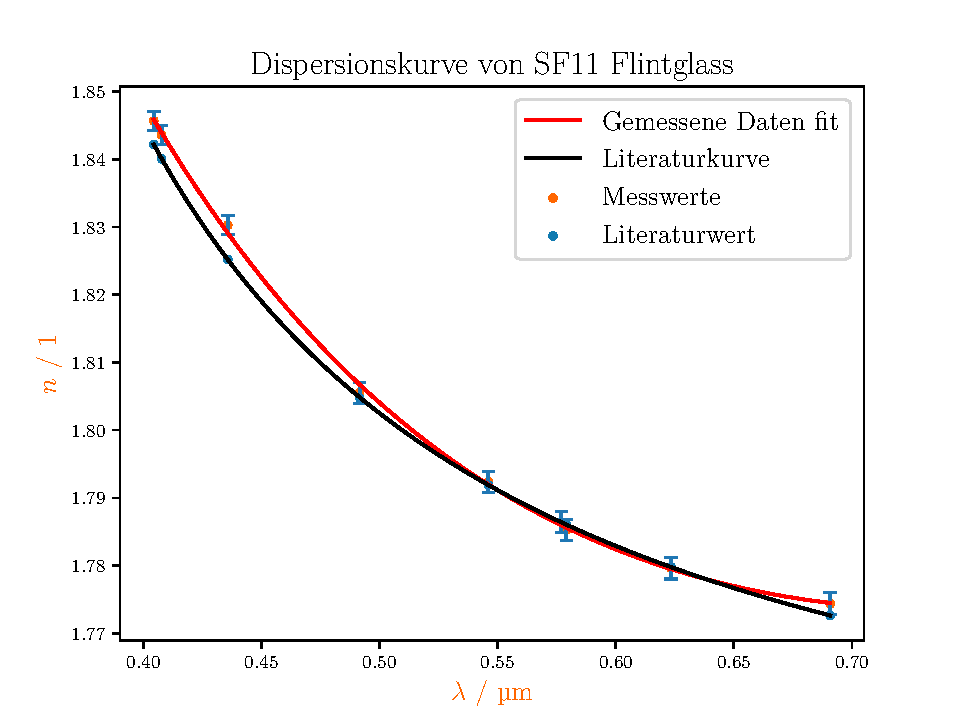
\includegraphics[width=0.95\textwidth]{./dispersion.pdf}
	\end{center}
	\caption{erhaltene Dispersionkurve}
	\label{fig:dispersionkurve}
\end{figure}

Die theoretische Kurve wurde ebenfalls geplottet mit:

\begin{equation}
	n^2-1=\frac{1.73848403\lambda^2}{\lambda^2-0.0136068604}+\frac{0.311168974\lambda^2}{\lambda^2-0.0615960463}+\frac{1.17490871\lambda^2}{\lambda^2-121.922711}
	\label{eq:theo_dispersionskurve}
\end{equation}


\subsubsection{Auflösungsvermögen}

Die Dispersion bei einer Wellenlänge von 0.0005791mm wurde aus der gefitteten Dispersionkurve gemessen, was folgende Werte liefert.

\begin{equation}
	\der{n}{\lambda}  = \SI{167.69(5)}{\per\mm}
	\label{eq:disperssionswert}
\end{equation}


Das Auflösungsvermögen bei einer Wellenlänge von \SI{0.0005791}{\mm} und einem $t=\SI{18.09(16)}{\mm}$ ist gleich der Dicke des Strahlbündels laut Tutor, was folgende Berechnungen ermöglicht:

\begin{equation}
	\frac{\lambda}{\Delta \lambda} = t \left| \der{n}{\lambda} \right|  = \num{3034(27)}
	\label{eq:auflosungprismawert}
\end{equation}



\section{Diskussion}\label{disk}

Die Winkelmessungen auf der linken und rechten Seite stellen sicher, dass eine Fehljustierung oder Verschiebung des Fadenkreuzes ausgeschlossen werden kann, da nur der Relativwinkel, als Differenz der beiden Messungen bei den darauf folgenden Berechnungen verwendet wird.

Auch ist die Gradmessung aufgrund des Nonius relativ genau gelungen. Diese könnte jedoch bei Verwendung eines Tisches mit genauerer Gradauflösung noch genauer sein.

Um die Unsicherheit zusätzlich zu verringern wurde immer von den 2. Beugungsordnungen aus gemessen.

Ein weiterer Verbesserungsvorschlag wäre computerunterstützte Messungen durchzuführen, um so beispielsweise den Umkehrpunkt für das Prisma oder die genaue Ausrichtung des Fadenkreuzes auf die Spektralen Linien noch genauer zu bestimmen. Diese würden dann über noch genauere Gradsensoren verfügen und so den entstehenden Messfehler deutlich senken.

Die Bestimmung des Durchmessers des Kollimatorrohrs konnte aufgrund des Millimeterpapiers als Maßstab sehr genau bestimmt werden.

\subsection{Gitter}

Der invertierte Wert der Gitterkonstante von \SI{572(4)}{\strich\per\mm} entspricht dem auf den Gitter angeschriebenen Wert von \SI{570}{\strich\per\mm}.

Vergleicht man die erhaltenen Werte aus \autoref{tab:wertwellenlange} mit den
angegebenen Werten aus der Vorlage \cite{gitterprismavorlage}, die in
\autoref{tab:wertbrechzahl} zu finden sind, ist sichtbar, dass alle erhaltenen
Werte außer ``Rot 1`` im Fehlerintervall enthalten sind. Dies ist
möglicherweise darauf zurückzuführen, dass der genaue Winkel bei rot nur sehr
schwer zu bestimmen war.

%Zusätzlich wurde die gesamte Berechnung nochmals mit der als Literaturwert gegebenen Gitterkonstanten von \SI{570}{\strich\per\mm} wiederholt, was folgende Werte liefert, die in folgender Tabelle den erhaltenen Werten gegenübergestellt werden.

% tab vgl

\subsection{Prisma}

Der erhaltene Wert für den brechenden Winkel des Prismas $\gamma$ sollte
aufgrund der Eigenschaften eines gleichseitigen Prismas \SI{60}{\degree}
betragen. \cite{Kuchling} Der Literaturwert ist also im erhaltenen
Fehlerintervall von \SI{59.8(10)}{\degree} enthalten.

\vspace{2mm}

Da zuerst davon ausgegangen wurde, dass der erhaltene Wert zu hoch sei, wurde nochmals alle Schritte durchgegangen, um mögliche Fehler ausfindig zu machen. Zusätzlich wurde Versucht durch Translationen die Grenzen der Fehler zu untersuchen, was schlussendlich zur Erkenntnis führte, dass die Durchführung nicht perfekt sein muss, um gute Werte zu erhalten.

Da so der vermeintliche Fehler nicht erklärt werden konnte, wurde der Versuch nochmals unter Verwendung eines anderen Prismas stichprobenartig durchgeführt, was jedoch auch die selben Werte lieferte.

\vspace{2mm}

Durch Gründliche Literaturrecherche wurde in Erfahrung gebracht, dass die Beschriftung des Prismas Aufschluss über das Material des Prismas gibt.

\begin{figure}[H]
	\begin{center}
		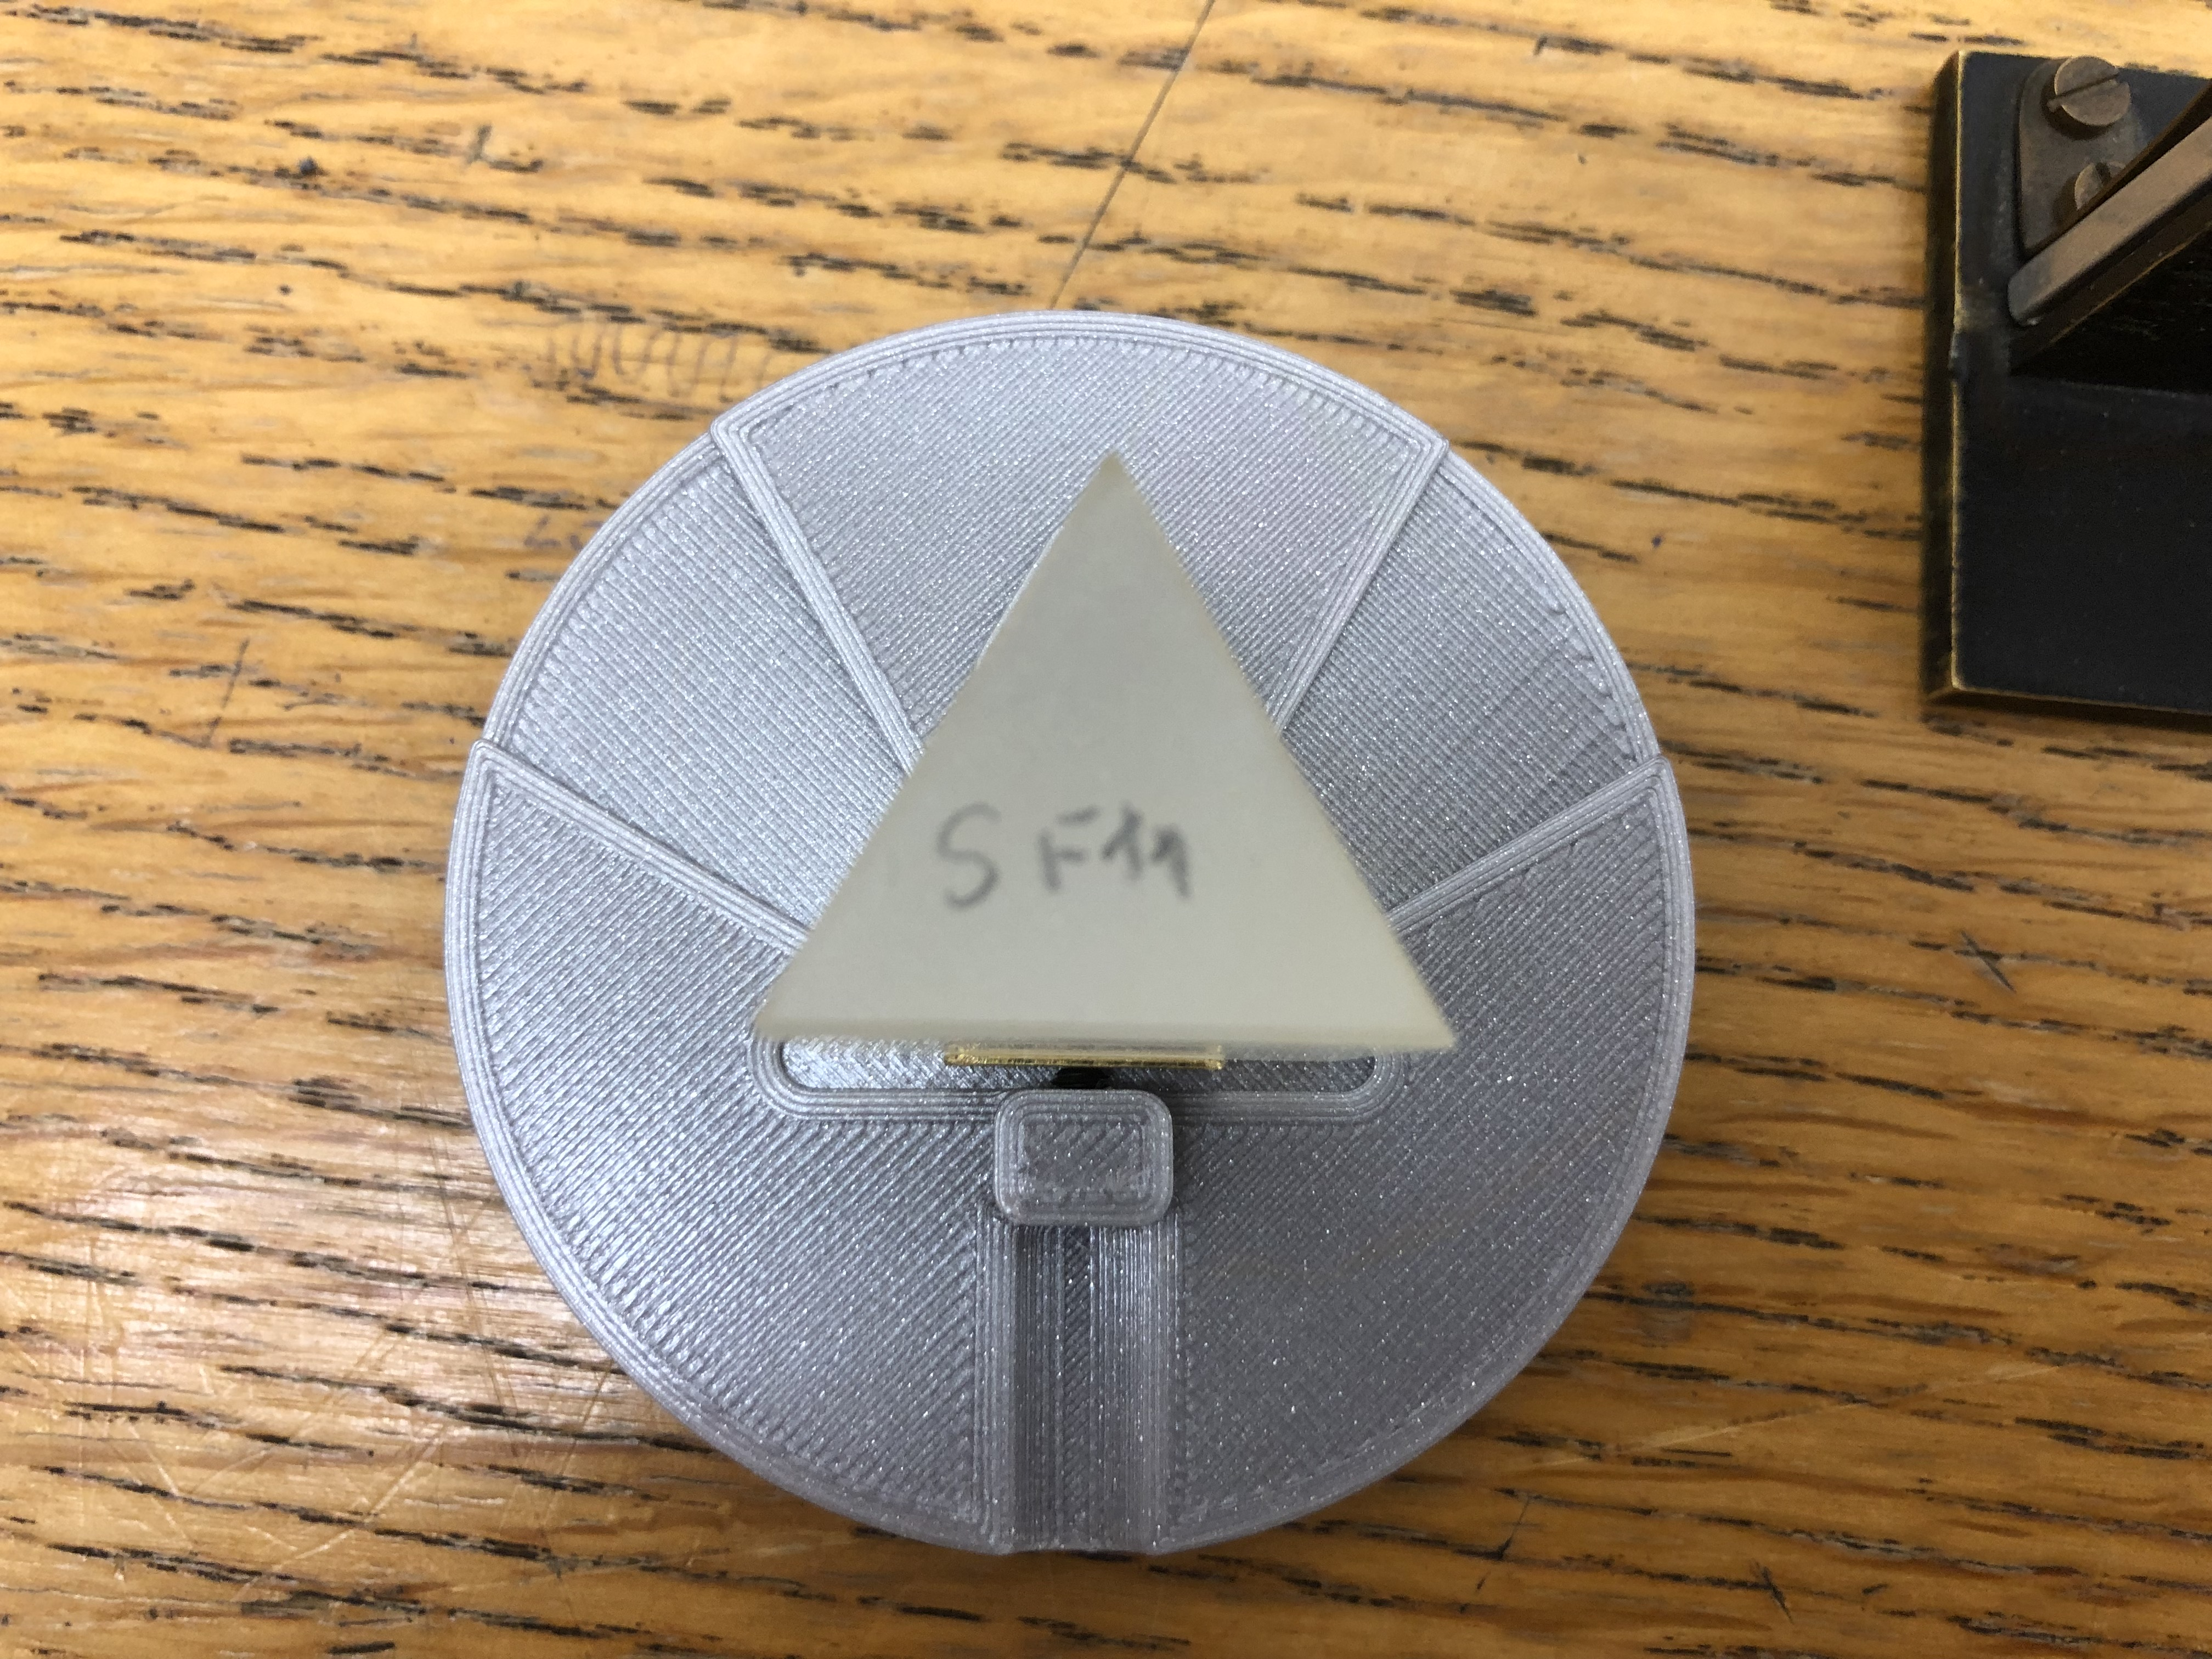
\includegraphics[width=0.5\textwidth]{prisma_fs}
	\end{center}
	\caption{Prisma mit Beschriftung anhand der das Material bestimmt werden kann}
	\label{fig:prisma_fs}
\end{figure}

Beim Material des Prismas handelt es sich um Flintglas SF 11 die entsprechenden
Brechungsindizes der jeweiligen Wellenlängen sind in
\autoref{tab:wertbrechzahl} den erhaltenen Werten gegenübergestellt.
\cite{brechzahl}


Dieser Vergleich zeigt, dass die erhaltenen Werte genau in der richtigen Größenordnung liegen und die Literaturwerte im Fehlerintervall enthalten sind.
Der Fit zeigt vor allem im mittleren Bereich eine große Übereinstimmung mit den Literaturwerten, die sogar in den Fehlerintervall enthalten sind. Für hohe und niederfrequente Bereiche weichen die erhaltenen Werte jedoch von der theoretischen Kurve ab.

\vspace{2mm}

Da die Kurve im Bereich von gelben Licht sehr gut mit der theoretischen Kurve übereinstimmt, kann die Dispersion bei diesen Wellenlängen, und dadurch auch das Auflösungsvermögen, sehr genau bestimmt werden, siehe \autoref{fig:dispersionkurve}.

\newpage

\section{Zusammenfassung}

\subsection{Gitter}

Für die Gitterkonstante $g$ wurde folgender Wert bestimmt:

\begin{align*}
	g = \SI{0.0017488(7)}{\mm}
\end{align*}

Anhand der Beugungswinkel wurden folgende Wellenlängen für die verschiedenen Farbeindrücke gemessen:

\begin{table}[H]
	\caption{Berechnete Wellenlängen für die verschiedenen Farbeindrücke \\ $\lambda \dots$ erhaltene Wellenlänge \\ $\Delta \dots $ entsprechende Unsicherheit}
	\centering
	\begin{tabular}{lrrrr}
		\toprule
		{}      & $\lambda$ / \si{\nm} & $\Delta \lambda$ / \si{\nm} \\
		\midrule
		Violett & 405                  & 3                           \\
		Blau    & 436                  & 3                           \\
		Türkis1 & 492                  & 3                           \\
		Türkis2 & 497                  & 3                           \\
		Grün    & 546                  & 3                           \\
		Orange1 & 577                  & 3                           \\
		Orange2 & 580                  & 3                           \\
		Rot1    & 608                  & 3                           \\
		Rot2    & 624                  & 3                           \\
		\bottomrule
	\end{tabular}
\end{table}

Für das Auflösungsvermögen des Gitters ergibt sich schließlich folgender Wert:

\begin{align*}
	\frac{\lambda}{\Delta \lambda} = \num{2.069(18)e+04}
\end{align*}

\newpage

\subsection{Prisma}

Für den Brechenden Winkel des Prismas $\gamma$ ergibt sich folgender Wert:

\begin{align*}
	\gamma = \SI{59.81(5)}{\degree}
\end{align*}

Für den Brechungsindex des Prismas ergeben sich folgende Werte:

\begin{table}[H]
	\caption{erhaltene Brechzahlen \\ $\lambda \dots$ gegebene Wellenlänge \\ $n \dots$ erhaltene Brechzahl  \\ $\Delta \dots$ entsprechende Unsicherheit}
	\centering
	\begin{tabular}{lrrrrrr}
		\toprule
		$\lambda$ / \si{\um} & $n$ / 1 & $\Delta n$ / 1 \\
		\midrule
		0.6908               & 1.7738  & 0.0011         \\
		0.6234               & 1.7796  & 0.0017         \\
		0.5791               & 1.7852  & 0.0016         \\
		0.5770               & 1.7864  & 0.0016         \\
		0.5461               & 1.7924  & 0.0016         \\
		0.4916               & 1.8055  & 0.0016         \\
		0.4358               & 1.8304  & 0.0015         \\
		0.4078               & 1.8436  & 0.0014         \\
		0.4045               & 1.8451  & 0.0013         \\
		\bottomrule
	\end{tabular}
\end{table}


Für das Auflösungsvermögen des Prismas ergibt sich schließlich folgender Wert:

\begin{align*}
	\frac{\lambda}{\Delta \lambda} = \num{3034(27)}
\end{align*}



\vspace{5mm}

\section{Anmerkungen}

Die ersten 3 Kapitel, sowie die dazugehörigen Abbildungen, wurden nicht von den
Autoren persönlich erstellt, sondern sind schon im Zuge der Aufgabenstellung,
in Form einer PDF, bereitgestellt und davon entnommen worden. \cite{gitterprismavorlage}

\newpage

\printbibliography
\listoffigures
\listoftables
\end{document}



%Vorlagen
%

%Gleichungen werden so oder mit \begin{equation} formatiert

%Zitate
%\cite{erstes Wort}


%Unterdrücken von Einrücken
%\noindent 

%referenzen
% \aotoref{name}

%für Formeln $ f $
%\subsection{Idealisierungen}

%Gleichung

%\begin{equation}
%	k_{pos} = \frac{4}{300} \frac{V}{\mu\mathrm{s}} = 13333 \, \frac{V}{s}
%\end{equation}

%\begin{align}
%	 \ddot \phi -\frac{g}{l} \cdot \phi &=0 \label{eq:harm}\\
%     \frac{\text{d}^{2}}{\text{dt}^{2}} [\sin(\omega t)]  - \frac{g}{l} \cdot \sin(\omega t) &= 0 \\ 
%     \therefore \quad \omega^{2}&=\frac{g}{l} \label{eq:omega}
%\end{align}


%\begin{align}
%    T &= 2\pi \sqrt{\frac{l}{g}} \label{eq:reg_sqrt} \\
%    T^{2} &= \frac{4\pi^{2}}{g} l \label{eq:reg_lin} 
%\end{align}

%Kompliziertes Bild

%\begin{minipage}{\textwidth}
%\begin{minipage}[t]{0.43\textwidth}
%	\includegraphics[width=\textwidth]{pics/toplot.PNG}
%\end{minipage}
%\begin{minipage}[t]{0.45\textwidth}
%	\includegraphics[width=\textwidth]{pics/bottomlot.PNG}
%\end{minipage}
%	\captionof{figure}{Ansicht von Oben (Rechts) und von Unten (Links) des Senklots}
%	\label{fig:Senklot}
%    \vspace{1em}
%\end{minipage}



%\begin{minipage}{\textwidth}
%\begin{minipage}[t]{0.59\textwidth}
%    \centering
%    \includegraphics[width=\textwidth]{pics/Aufhangung.jpeg}
%    \captionbelowof{figure}{Aufhängung}
%    \label{fig:Aufhaengung}
%\end{minipage}
%\begin{minipage}[t]{0.40\textwidth}
%    \centering
%    \includegraphics[width=\textwidth]{pics/PendelAufbau.png}
%    \captionof{figure}{Versuchsaufbau}
%    \label{fig:Aufbau}
%\end{minipage}
%    \vspace{1em}
%\end{minipage}

%\begin{wrapfigure}[]{r}{0.4\textwidth}
%\begin{tabular}{@{}l@{}}
%\begin{minipage}{\textwidth}
%\includegraphics[width=0.38\textwidth]{pics/Aufhangung.jpeg}
%\noindent \captionbelowof{figure}{Aufhängung}
%\label{fig:Aufhaengung}
%\end{minipage}\\
%\begin{minipage}{\textwidth}
%\includegraphics[width=0.38\textwidth]{pics/PendelAufbau.png}
%\captionof{figure}{Versuchsaufbau}
%\label{fig:Aufbau}
%\end{minipage}
%\end{tabular}
%\end{wrapfigure}


%Tabelle

%\begin{align}
%	\Delta \bar T_{10} &= t \sigma_{\bar T_{10}} + \Delta T_{res} = \frac{t}{\sqrt{N}}\sigma_{T_{10}}+\Delta T_{res}\\
%	\Delta \bar T &= \frac{ \Delta \bar T_{10}}{10}
%\end{align}


%Tabelle
%
%\begin{table}[htbp]
%\centering
%\begin{tabular}{c|c|c|c|l}
%    [$\frac{\text{m}}{\text{s}^{2}}$] & Literaturwert & Wurzel Fit & Linearer Fit &\\ \hline
%    $g$ & \num{9.806191} & \num{9.79} & \num{9.80} &\\
%    $\Delta g$ & \num{1.2e-5} & \num{1e-2}& \num{1e-2} &\\
%\end{tabular}
%	\captionbelowof{table}{Vergleich mit Literaturwert}
%	\label{Tab:Vergleich}
%\end{table}


%\begin{align}
%	& \Delta T_{\phi} = 2\pi \sqrt{ \frac{l}{g} } \frac{\phi^{2}}{16} = 0.0052\,\text{s} 
%\end{align}
